\documentclass[10pt, nofootinbib, twocolumn]{revtex4-1}
\usepackage{amsmath}
\usepackage{xparse}
\usepackage{graphicx}
\usepackage{hyperref}
\usepackage{color}
\usepackage{physics}
\usepackage{enumitem}
\usepackage{natbib}
\usepackage{booktabs}
\usepackage{float}
\usepackage{caption}
\hypersetup{
    colorlinks=true,
    linkcolor=black,  
    citecolor=black,
    urlcolor=blue
}

\begin{document}
\vspace*{2\baselineskip}
\title{The 2D Ising Model : Behaviour Around Equilibrium} 
\author{Tiril Sørum}\homepage{https://github.com/tirilsg/FYS3150-Project4}
\date{\today}        
\begin{abstract}
\vspace*{1\baselineskip}
    \textit{The two-dimensional Ising Model for fixed lattices of spins with periodic boundary conditions is implemented in this report, and by utilizing the Monte Carlo based Metropolis algorithm, we manage to simulate its behaviour in different environments. Our algorithm works in such a way that it calculates the expected values for energy and magnetization, as well as heat capacity $C_V$ and magnetic susceptibility $\chi$ for each cycle it performs. We check our model's correctness by simulating the temperature-dependent behaviour of both $2\times 2$ and $20\times 20$ lattices, and find both a large conformity between the  model and our expected results, and a number of $10^4$ needed Monte Carlo cycles performed for the system to reach equilibrium, independent of initial condition of spins and temperature. To make sure equilibrium was reached for the rest of our simulations, an amount of  $10^5$ cycles were used. The critical temperature obtained numerically by the $20\times 20$ lattice simulation was estimated to about $T=2.3J/k_B$, which when compared with the expected $T_C=2.269J/k_B$ displays a large degree of precision. The data for these simulations were used to display the probability distribution, which was in agreement with both the rest of our modelled data, and our expectations with ground in theory presented in this report. Furthermore, simulations of the behaviour of lattices with an increasing lattice size was conducted, in which the data was used to estimate critical temperatures for each of these cases of lattice sizes. These simulations were performed by making use of parallelization, which we found to make the simulations run a total of 3.73 times faster than simulations ran without taking advantage of this method. Seeing these estimated temperatures in light of expected temperature-lattice size relations, left us with an ultimate estimation of critical temperature $T_C = 2.252\pm 0.008J/k_B$, which is found to have a good degree of accuracy when comparing it to the expected value $T_C=2.269J/k_B$.}
\end{abstract}
\maketitle       


\section{Introduction}\label{sec:introduction}
The Ising Model is an excellent tool to make use of when investigating physical properties of magnetic materials. It is an incredibly simplified model of reality, that in spite of its simplicity describes the behaviour of a fixed, lattice structured material in such a way, that it offers a window into the quantum world of spin interactions. The conditions on which the model is built upon, makes it possible for us to study the physical processes happening within such systems during phase transitions, even if the size becomes quite large. \\

By implementing this model, one can study how the behaviour of such a lattice - with periodic boundary conditions for simplicity - changes as a response to thermal energy. A system of this sort is in accordance with the first law of thermodynamics, continuously striving towards a state of equilibrium. This state is expected to be reached at a point that we refer to as the \textit{critical point}, which is characterized by the \textit{critical temperature} $T_C$, and the abrupt change of behaviour of the spontaneous magnetization our system exhibits. Thereby we can study how the behaviour of such system changes with temperature, to gain a broader understanding of what processes takes place when approaching this critical temperature. \\

In this report, we study the intricacies of this model by deploying the Monte Carlo based Metropolis algorithm so simulate the behaviour of such magnetic systems around the critical temperature. We begun by comparing the modelled behaviour of a $2\times 2$ lattice structure with analytic expressions we derive for the specific situation. From there we studied larger size lattices, starting with $20\times 20$ lattices in different environments, and studying how these different conditions affected the observed behaviour. Both simulations of $2\times 2$ and $20\times 20$ lattices ensured the model's correctness and accuracy for the investigation of phase transitions to come. \\

By taking advantage of parallelization of our code to ensure optimal efficiency, we simulated the behaviour of latices of different sizes over different temperatures around the critical point. Our goal; using the modelled behaviour to create a link between the temperature change and size of the lattices, ultimately contributing to a deeper understanding of the processes occurring.


\newpage
\section{Theory}\label{sec:theory}
\subsection{The Ising Model}\label{sec:Ising}
The Ising model describes a system which consists of N spins $s_i$ in a fixed lattice structure of size $L \times L$, where each spin only exists in one of two possible conditions; $\downarrow s_i=-1$ and $\uparrow s_i=+1$, spins up and down. The model applies periodic boundary conditions to these spins, meaning we limit the interactions happening between spins to only occur between spins situated left, right, up and down from each other - meaning all spins $s_i$ essentially only have four neighbors. We describe the energy within this system as a sum of interactions between each-spin's neighboring spins, without any double counting, expressed by the formula 
\begin{equation}\label{eq:en1}
E(\mathbf{s}) = -J \sum\limits_{\langle kl \rangle}^{N} s_k s_l
\end{equation}
where J is referred to as the coupling constant, and N is the total amount of spins within the entire system \cite[p.~194]{stats}. $\langle kl \rangle$ indicates that we only sum over neighboring spins. The size of coupling constant $J$ does take into consideration the effect of the magnetic field set up by each spin, as well as coupling between the field and spin and decay with distance. Subsequently, we can look at J as an annotation of the strength of interaction between spins. By summing over all of the spins in the system, we obtain an important unit that we call magnetization:
\begin{equation}
 M(\mathbf{s}) = \sum\limits_{i}^{N} s_i
\end{equation}




\subsection{Statistical Mechanics}
The particles that make up the material who's structure we model by the Ising Model, cannot have position and velocity precisely determined by mathematical formulas. By using statistics to model a system consisting of particles of many degrees of freedom, one can derive expressions using probability of finding a system of particles in a certain sate at a certain time. For a system at equilibrium, this probability is described by \textit{Boltzmann probabilities} \cite[p.~184]{stats}
\begin{equation}
    P(E_i)= \frac{1}{Z}e^{-E_i/k_BT}, \label{eq:probfunc}
\end{equation}
where $k_B$ is Boltzmann's constant, $E_i$ is the energy of the state $i$, T is the temperature, and $Z$ is what we refer to as the \textit{partition function}, and is defined
\begin{equation}
    Z(N,V,T)= \sum_{i}e^{-E_i/k_BT} = \sum_{e_l s}g(E_s)e^{-E_i/k_BT} , \label{eq:partitionfunc}
\end{equation}
where N is the number of different states of the system. We refer to $g(E_s)$ as the degeneracy, where $e_l s$ is the energy levels s.
We can use the partition function \eqref{eq:partitionfunc}, to further deduce formulas describing the system of the Ising Model, including expected values for energy $\langle E \rangle$ and magnetization $\langle M \rangle$.
\begin{equation}
    \langle E \rangle = \frac{1}{Z}\sum_{i=1}^{N}E_ie^{-E_i/k_BT}, \label{eq:ene}
\end{equation}
\begin{equation}
     \langle M \rangle = \frac{1}{Z}\sum_{i=1}^{N}M_ie^{-E_i/k_BT}, \label{eq:mag}
\end{equation}
$\langle E^2 \rangle $ and $\langle M^2 \rangle$ can be calculated by inserting these values $E_i^2$ and $M_i^2$ into the Equations \eqref{eq:ene} and \eqref{eq:mag} as replacement for $E_i$ and $M_i$. The Equations \eqref{eq:ene} and \eqref{eq:mag} can also be used to calculate standard deviation of both the expected energy and magnetization, and thereafter express heat capacity $C_V$ magnetic susceptibility $\chi$. 
\begin{equation}
    C_V = \frac{1}{k_B T^2}(\langle E^2 \rangle - \langle E \rangle^2) = \frac{1}{k_B T^2} \sigma_E \label{eq:heat}
\end{equation}
The heat capacity $C_V$ \eqref{eq:ene} is a measurement of the heat/energy required to change the temperature of a volume $V$, or in the case of a 2D system $A$, of matter by one degree. This variable can also be defined as the integral of the average energy $\langle E \rangle$ with respect to temperature $T$. 
\begin{equation}
    \chi = \frac{1}{k_B T}(\langle M^2 \rangle - \langle |M| \rangle^2) = \frac{1}{k_B T} \sigma_M \label{eq:sus}
\end{equation}
The magnetic susceptibility $\chi$ \eqref{eq:sus} is a measurement of how much, and to what degree a material will become magnetized by an applied magnetic field. This variable is a constant, analogous to heat capacity, for the volume of material within a system. \\The thermodynamical potential of our system is described by Helmholtz' free energy \cite[p.~430]{notes}
\begin{equation}
    F = \langle E \rangle - TS = -k_bTln(Z) \label{eq:ther}
\end{equation}
This equation is important, as it relates the expectation value for energy at the temperature $T$, to the entropy $S$, or degree of randomness within the system, at the same temperature. It is explained to express the struggle between two important principles in physics \cite[p.~419]{notes} - the strive towards an energy minimum and the drive towards higher entropy as the temperature increases. At equilibrium, \eqref{eq:ther} will balance. 

\newpage
\subsection{Phase Transition}
Temperature-dependent behaviour in the Ising Model, is especially interesting at the point $T=T_C$, which we refer to as the \textit{critical temperature}. This critical point is marked by abrupt macroscopic changes, which this means a small change in spins will result in a large change in behaviour. The behaviour around this critical point can be related  to different derivatives of the thermodynamic potential \eqref{eq:ther}, by rewriting the Equations \eqref{eq:ene} and \eqref{eq:mag}. We have for temperatures lower than the critical temperature $T_C$: 
\begin{equation}
    \langle M \rangle \sim \left(T-T_c\right)^{1/k_BT} \label{eq:critm}
\end{equation}
where the variable $1/k_BT$, or the Boltzmann's constant $\beta$ is equal to $1/8$. One can deduce the same type of relation for both the heat capacity and magnetic susceptibility for a temperature lower than $T_C$: 
\begin{equation}
    C_V \sim \abs{T_c-T}^{-\alpha} \label{eq:critcv}
\end{equation}
\begin{equation}
    \chi \sim \abs{T_c-T}^{-\gamma} \label{eq:critchi}
\end{equation}
here $\alpha = 0$ and $\gamma=-7/4$, and are along with $\beta$, as critical exponents. Both \eqref{eq:critcv} and \eqref{eq:critchi} will in theory diverge near $T_C$, but when dealing with a finite lattice this behaviour will not occur. Quite the opposite, in fact; the heat capacity $C_V$ will have a maximum near the critical temperature $T_C$ instead \cite[p.~431]{notes}. \\

As T approaches $T_C$, another variable we introduce called correlation length $\xi$, increases and as long as our system is a finite lattice ($L \times L$) of second order, will approach L
\begin{equation}
    \xi  \sim |T_C - T|^{-\nu} \label{eq:xi}
\end{equation}
One can relate the behaviour of finite lattices with lattices that are infinite large ($L \longrightarrow \infty$) by scaling the critical temperatures 
\begin{equation}\label{eq:corr}
  T_C(L) - T_C(L=\infty) \propto aL^{-1/\nu}.
\end{equation}
where $a$ is a constant, and $\nu$ is defined by the Equation \eqref{eq:xi}, and thereby 
\begin{equation}
    \xi \propto L \sim |T_C - T|^{-\nu} \label{eq:xiinf}
\end{equation}
By setting $T=T_c$, we can use this correlation for lattice spacing, to derive the following L-dependent relations, from Equations \eqref{eq:critm}, \eqref{eq:critcv} and \eqref{eq:critchi}: 
\begin{align}\label{eq:relations}
    \begin{split}
        \langle M \rangle &\propto L^{-\beta/\nu} \\
        C_V &\propto L^{\alpha/\nu} \\
        \chi &\propto L^{\gamma/\nu}
    \end{split}
\end{align}


\subsection{Analytical Results for Special Case} \label{sec:analytical}
To ensure that the coding for our Ising Model is as accurate as possible, comparisons between modelled and analytical values is necessary. Subsequently, the deduction is done for the following expressions, for a $2\times 2$ lattice system with periodic boundary conditions, using Equations \eqref{eq:partitionfunc}, \eqref{eq:ene}, \eqref{eq:mag}, \eqref{eq:heat} and \eqref{eq:sus}
\begin{align}
& Z=4cosh(8J\beta)+12 \label{eq:anpar} \\
& \langle E \rangle = \frac{16J e^{-8J\beta}}{Z} = \frac{-32J\sinh{\left(8J\beta\right)}}{Z} \label{eq:anene} \\
& \langle E^2 \rangle = \frac{256J^2\cosh{\left(8J\beta\right)}}{Z} \label{eq:anene2} \\
& \langle \abs{M} \rangle = \frac{64 + 64e^{8J\beta}}{Z} = 8\frac{2 + e^{8J\beta}}{Z}  \label{eq:anmag} \\
& \langle M^2 \rangle = \frac{256 + 256e^{8J\beta}}{Z} = 32\frac{1 + e^{8J\beta}}{Z} \label{eq:anmag2} \\
& C_V = \frac{\beta}{T}\left(\frac{256J^2\cosh{\left( 8J\beta \right)}}{Z} - \left(\frac{-32J\sinh{\left( 8J\beta \right)}}{Z}\right)^2\right)  \label{eq:ancritchi} \\
& \chi = \beta\left(32\frac{1+e^{8J\beta}}{Z} - \left(8\frac{2+e^{8J\beta}}{Z}\right)^2\right) \label{eq:ancritchi2} \\
\end{align}
The deduction, as well as visualization of the structure of the Ising model itself, can be viewed in the Appendix \ref{sec:appendix} attached to the report. 


\cleardoublepage
\section{Algorithm}\label{sec:algorithm}
\subsection{The Metropolis Algorithm}
The simulation of the Ising model is done by utilizing the Monte Carlo based Metropolis algorithm \cite[p.~435]{notes}. By doing so, one can avoid having to make use of the partition function \eqref{eq:partitionfunc}, which would involve computations for every single possible state $2^N$ and thereby make our program challenging to run effectively. Instead, this algorithm makes use of rations between energy-dependent transition probabilities \eqref{eq:ene}. The algorithm goes as follows: 
\begin{center} ------------------------------------------------------------ \end{center}
\begin{description}[]
    \item \textbf{Construction of an initial state} with an energy $E_0$ at a random position in the lattice. 
    \item \textbf{The configuration is changed} by flipping a single spin, and the change in energy $\Delta E=E_1-E_0$ is calculated. 
    \item \textbf{Determine whether} $\Delta E \leq 0$ or $\Delta E>0$. If $\Delta E \leq 0$, we're moving closer to the critical point, and the new configuration (redefined by the recently flipped spin) is accepted. An $\Delta E>0$ means the new configuration only is accepted if $e^{-(\beta \Delta E)} \geq r$ where r is a random number between 0 and 1. If this condition is not met in this case, the old configuration (before the spin was flipped) is kept. We use an expression deduced from our Equation \ref{eq:en1}: $\Delta E = 2Js_l^1 \sum_{\langle kl \rangle}^{N}s_k$ \cite[p.~438]{notes}.
    \item \textbf{Interesting expectation values are updated}. In our case, these values include $E$, $E^2$, $\abs{M}$, $M^2$ calculated by \eqref{eq:ene} and \eqref{eq:mag}. 
    \item \textbf{The cycle of flipping spins} is looped and repeated, until an adequate amount spins have been selected. The amount of spins selected can be adjusted as to what degree of accuracy we wish to approximate the critical point and the corresponding expectation values. 
\end{description}
\begin{center} ------------------------------------------------------------ \end{center}
We refer to the process of repeatedly flipping a spin and calculating updated expectation values as a \textit{Monte Carlo cycle}. During each of these cycles, one calculates the expectation values, which can be extracted and used to create various plots that visualize the convergence as the critical point is approached. 



\newpage 
\section{Methods}\label{sec:methods} 
\subsection{Theory Comparison}
While developing the code, we undergo continuous tests to make sure the code works to the best degree possible. We make use of the analytical expressions for the instance of a lattice size $2\times 2$ presented in section \ref{sec:analytical}, and compare the modelled data with these expressions. This way, we make benchmarks for our code, and can the same way undergo an error analysis to make sure any inaccuracies are sufficiently small, before making use of the Ising Model to discuss the behaviour of lattices of larger sizes. 


\subsection{Code Efficiency}
A simple method we make use of to make our calculations and simulations less time consuming, is scaling our equations by assigning units $J$ and $k_B$. Subsequently, energy will be expressed in units of J, magnetic susceptibility 1/J, temperature $k_B/J$, and heat capacity $k_B$ - something which simplifies our Equations \ref{eq:ene}, \ref{eq:mag}, \ref{eq:heat} and \ref{eq:sus} significantly. By setting both $k_B$ and $J$ equal to 1, we both generalize and simplify our simulation. \\

We take advantage of a number of fortunate conditions when developing our model, to make sure it runs as smooth and effortlessly as possible. One of these conditions is a consequence of the \textit{periodic boundary conditions}. As described in section \ref{sec:Ising}, each particle in the 2D lattice structured Ising model will only be able to interact with four neighboring particles, which simplifies our formulas describing the environment within the system. An important consequence of the \textit{periodic boundary conditions} is; there are only five unique energy states our system can assume when the Metropolis Algorithm \ref{sec:algorithm} flips a spin in positive direction, $\Delta E = -8J, -4J, 0J 4J$ and $8J$ \cite[p.~436]{notes}, which reduces the amount of operations necessary for simulation drastically. Furthermore, only the unique energy states will be described by a Boltzmann constant $e^{E_i/k_BT}$ that does not equal 0. We take advantage of this when developing code, to make simulations run as efficiently as possible. \\

To further improve the efficiency of our code, we make use of a method called parallelization. By parallelizing our code, we're able to run simulations and collect data for otherwise overly time consuming situations. This is done by making use of the c++ library $<omp.h>$ OpenMP, and thereby enabling the simulation to run simultaneously on four different processors. This is extremely convenient when we wish to run simulations for lattices of larger sizes, over an interval of different temperatures. When compiling the files making use of this parallelized code, it is important to remember to add the flag $-fopenmp$ when compiling. 


\subsection{Simulation}
The accuracy of our model is evaluated by simulating the behaviour a $2\times 2$ lattice around the critical point, and comparing expectation values with the analytical expressions presented in section \ref{sec:analytical}. \\

To study the behaviour of lattices modelled by the Ising Model, we run simulations with different environmental conditions. One of these conditions concerns our initialization of the spins within our system, which we examine by simulating systems where every spin is initialized in the same direction (up $\uparrow $), as well as systems where every spin is randomly assigned a direction of spin (up $\uparrow$ or down $\downarrow$). To initialize the spins in random directions, we use the Mersenne Twister generator $(mt19937)$. By interpreting data collected by running simulations for systems with different initialized spins at different temperatures, we can determine how many many times we need to run our Metropolis Algorithm before equilibrium is reached for our system. We use this to make sure our simulations acquire data that is accurate enough to use as base for any conclusions. \\ 

By investigating how modelled expectation values changes by temperature and lattice size, we can both further investigate the accuracy of our model, and relate the behaviour to the Equations \ref{eq:relations} for temperature-lattice size relations around the critical temperature. Furthermore, by creating functions for heat capacity $C_V$ from our data, and  extracting the temperature in which the heat capacity is at an apex, we can obtain a modelled value for the critical temperature for a lattice of an arbitrary size. By investigating how this modelled critical temperature changes with increasing lattice size, and comparing it to the expected value 
$$T_C=2.269185[k_B/J]$$
introduced by \textit{Ulli Wolff} in 1989 \cite[p.~448]{notes}, we can draw further conclusions regarding both the occurring phase transitions, and the accuracy of our model.



\cleardoublepage 
\section{Results}\label{sec:results}
\subsection{Theory comparison}
The Ising Model is tested for our $2\times 2$ lattice, and compared to the expressions \eqref{eq:anpar} - \eqref{eq:ancritchi2}, to make sure it works as intended, and with an appropriate degree of correctness. To do so, we calculate the expectation values for both varying temperatures in the interval $T\epsilon [0.5,4]J/k_B$, and for varying amounts of Monte Carlo cycles $10, 10^2 10^3, 10^4$ and $10^5$. 
To show how the precision in calculation of expectation values increases with an increasing amount of Monte Carlo cycles performed by our algorithm, these results are presented in a scatter-plot Figure \ref{fig: fig2}, as well as in the Table \ref{tab:mcerr}. The estimation of the relevant expectation values for an amount $10^5$ of Monte Carlo cycles is presented in Figure \ref{fig: fig1}. \\

\begin{figure}[H]
    \centering
    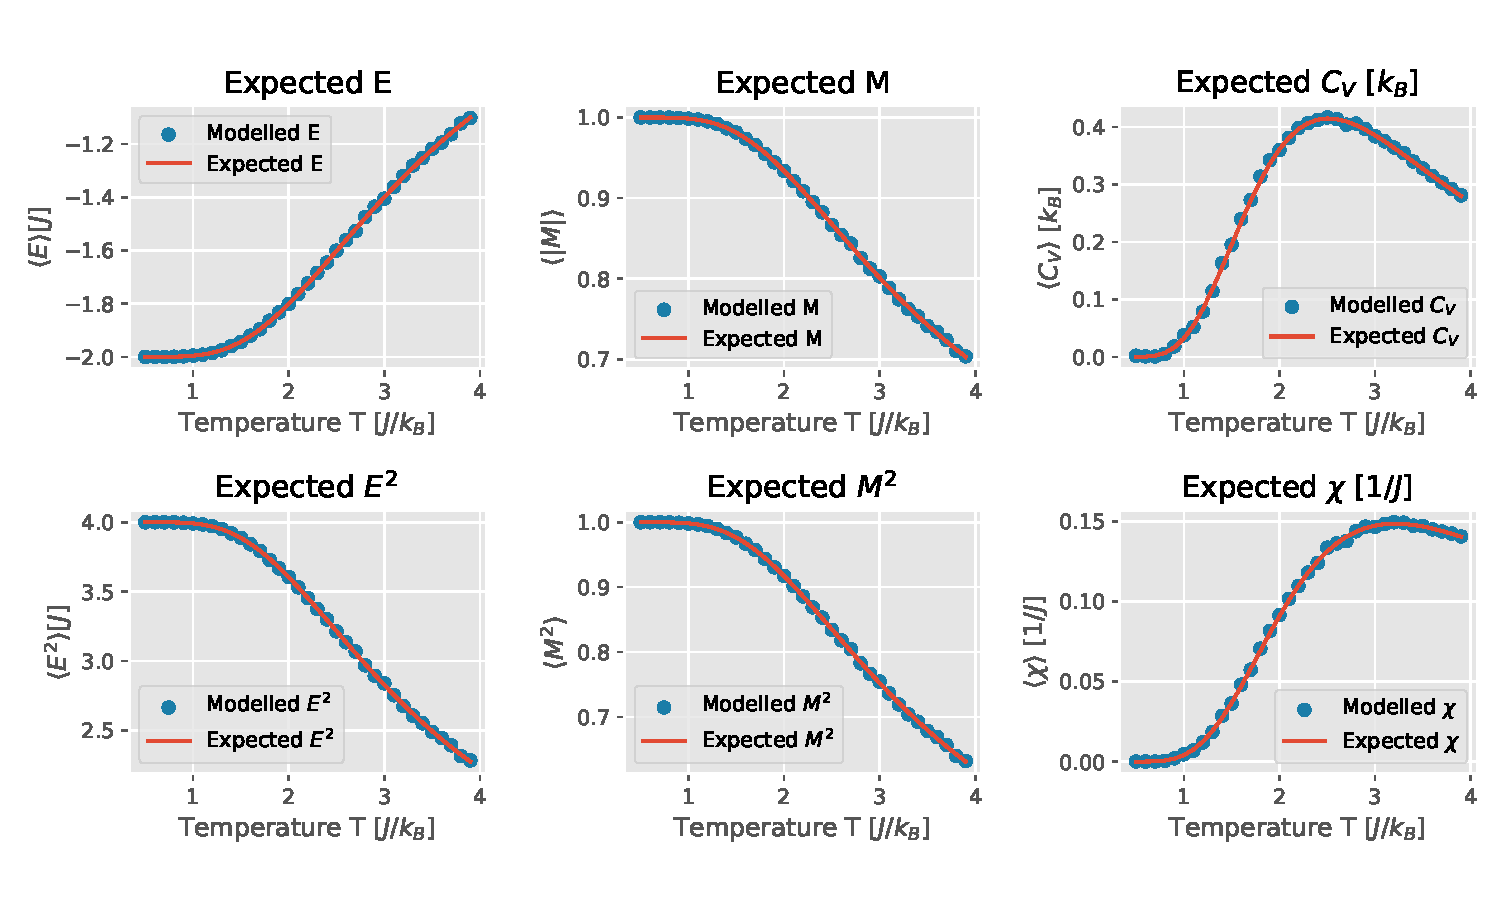
\includegraphics[width = 1\textwidth]{figures/expected_values.pdf} 
    \caption{Visualizing and comparing the numeric and analytic estimation for the expectation values in the special case of a $2\times 2$  lattice, for an amount $10^5$ of Monte Carlo cycles, over an interval of temperature $T\epsilon [0.5,4]J/k_B$ with temperature steps dT=0.1$J/k_B$. Analytic expressions presented by Equations \ref{eq:anpar} - \ref{eq:ancritchi2} in section \ref{sec:analytical}.}
    \label{fig: fig1}
\end{figure} 

\newpage

%MC Cycles:       Average relative error E:     Average relative error abs(M):
%10               0.5925372461637285             0.16289832623461023
%100               0.21357392579212928             0.08225180883285868
%1000               0.0752367425994386             0.025830585185352004
%10000               0.03237745213753096             0.011508111198174095
%100000               0.009075830256436771             0.003057848212326559


\begin{center}
    \begin{table}[h]
    \caption{Estimated expectation values for the lattice of size $2\times 2$, with an increasing amount of Monte Carlo cycles performed by simulation. The error is an average over all the temperatures in the interval our simulation is ran for, $T\epsilon [0.5,4]J/k_B$. How the error varies with temperature in the case of $10^5$ Monte Caro cycles can be viewed in Figure \ref{fig: fig1onlyerrors}, attached to the Appendix \ref{sec:appendix}.} 
        \begin{tabular*}{0.5\textwidth}{@{\extracolsep{\fill}}ccc}
        \toprule
        \hline \\
        MC Cycles:    &   Relative error E:   &  Relative error abs(M): \\
        \midrule
        \hline \\
        $10$       &        0.593      &     0.163 \\
        $10^2$      &         0.214     &      0.0823 \\
        $10^3$      &        0.075    &       0.0258 \\
        $10^4$      &         0.032    &         0.0116 \\
        $10^5$        &        0.0091    &        0.00306 \\
        \hline
        \bottomrule
        \end{tabular*}\label{tab:mcerr}
    \end{table}
\end{center}



\begin{figure*}
    \centering
    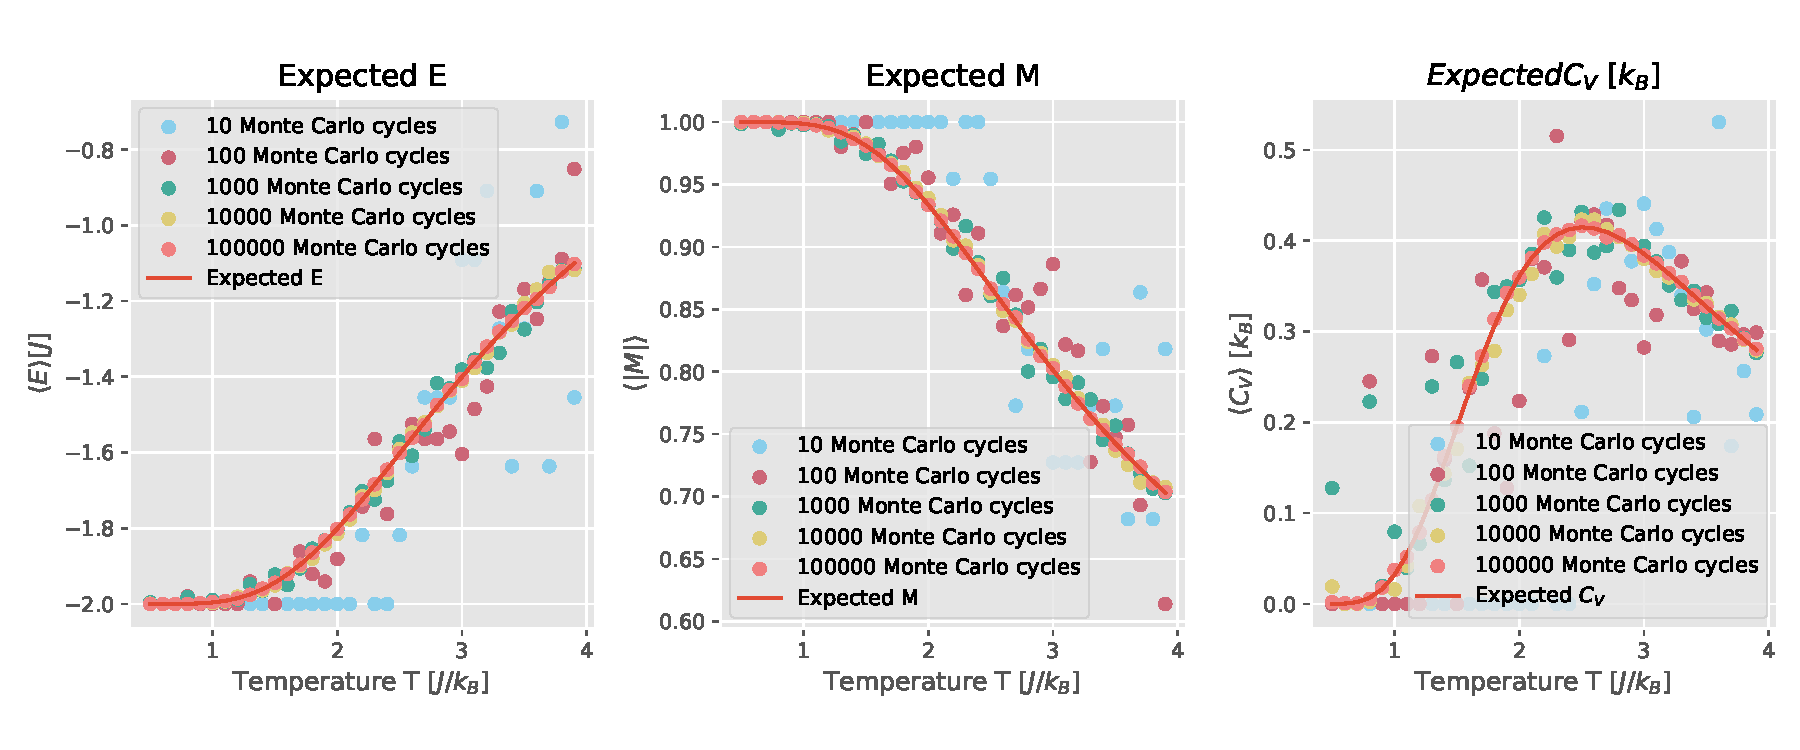
\includegraphics[width = 1\textwidth]{figures/mcc_comp.pdf} 
    \caption{Degree of precision for the expectation values of energy (left), absolute magnetization (middle) and heat capacity $C_V$ (right), for varying amounts of Monte Carlo cycles used for estimations. For a visualization of the behaviour of every expectation value, see Figure \ref{fig:all} in the Appendix \ref{sec:appendix}. The expectation values are estimated over an interval of temperature $T\epsilon [0.5,4]J/k_B$ with temperature steps dT=0.1$J/k_B$.}
    \label{fig: fig2}
\end{figure*} 

\newpage
\subsection{The $20\times 20$ Lattice}
We use a lattice of size $20\times 20$ to investigate modelled behaviour at temperatures $T=1J/k_B$ and $T=2.4J/k_B$. By visualizing how the expected energy and expected absolute magnetization changes with amounts of Monte Carlo cycles, we can determine how many cycles are needed to obtain an equilibrium for our systems. These models are created for initial conditions of both randomly generated spin (either positive $\uparrow$ or negative $\downarrow$), and spin initialized in the same direction (positive $\uparrow$), and visualized in Figure \ref{fig:cycleamount}. From this Figure, one can read that there's an equilibrium obtained around $10^4$.
\begin{figure*}
    \centering
    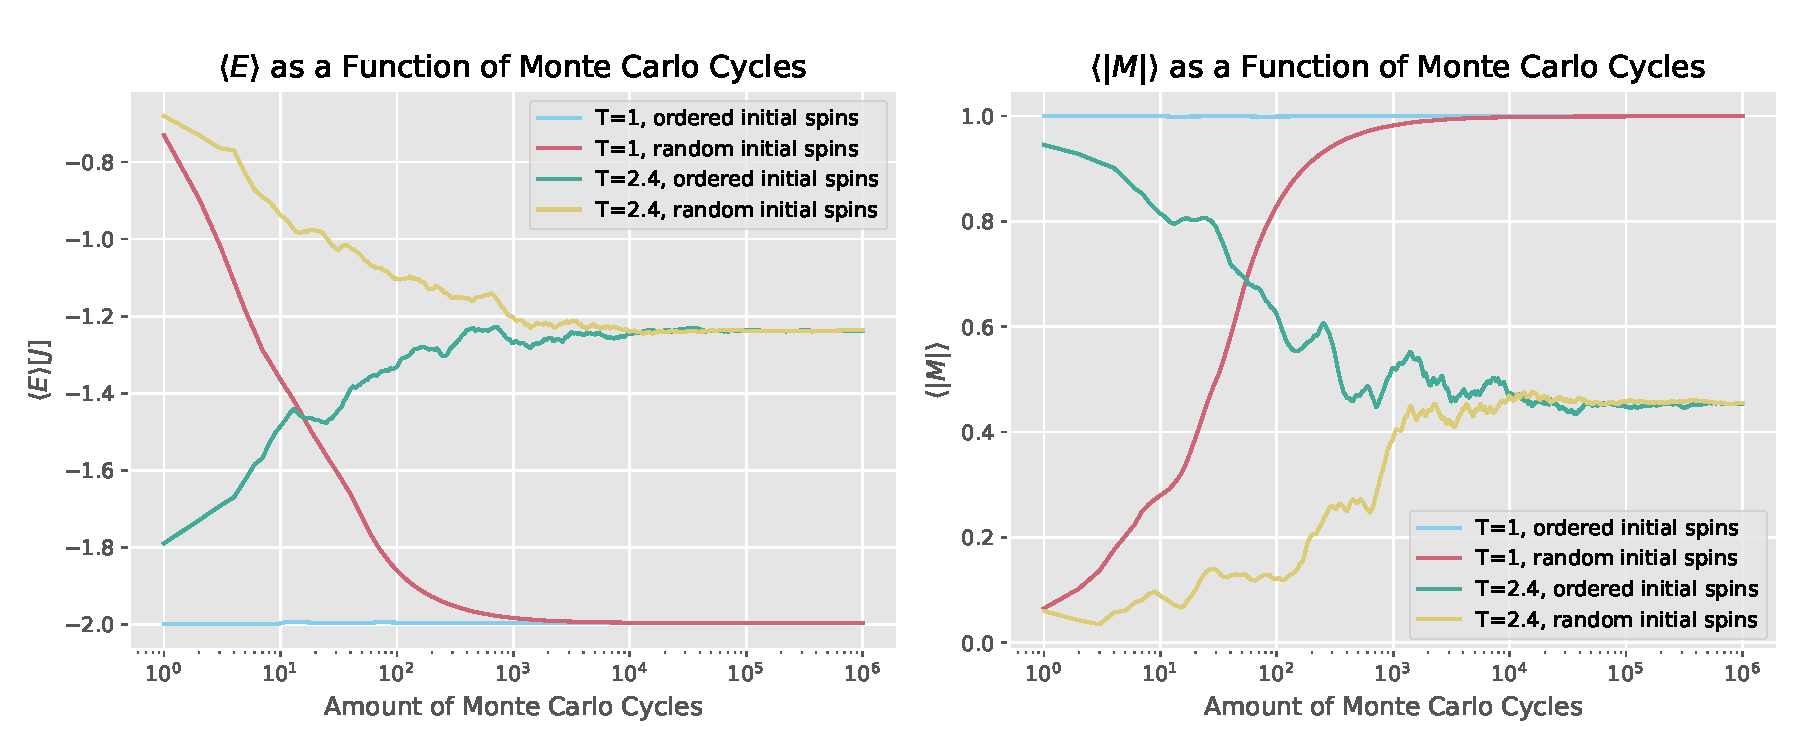
\includegraphics[width=1\textwidth]{figures/20x20randord.pdf} 
    \caption{Evolution of expected value for energy (left) and magnetization (right) for $T=1J/k_B$ and $T=2.4J/k_B$ as a function of Monte Carlo cycles performed by the simulation, initialized in both random and fixed (ordered in positive spin direction) directions. The lattice size is $20\times 20$.}
    \label{fig:cycleamount}
\end{figure*}
Furthermore, we use simulation of the $20\times 20$ lattice size for a varying temperature in the interval $T\epsilon [0 , 6] J/k_B$ and steps in temperature calculations dT = 0.1$J/k_B$ to show percent of accepted flips as a function of this temperature. This data is visualized in Figure \ref{fig:acceptedflips}. \\

By using histograms showing how often a certain energy is registered in our model, we can visualize the probability distribution function for the model. This technique is used for a lattice of size $20\times 20$, for both temperatures $T=1J/k_B$ and $T=2.4J/k_B$ that had random initialization of spin, and we get the Figures \ref{fig:frac} and \ref{fig:perc}. 

\newpage
\begin{figure}[H]
    \centering
    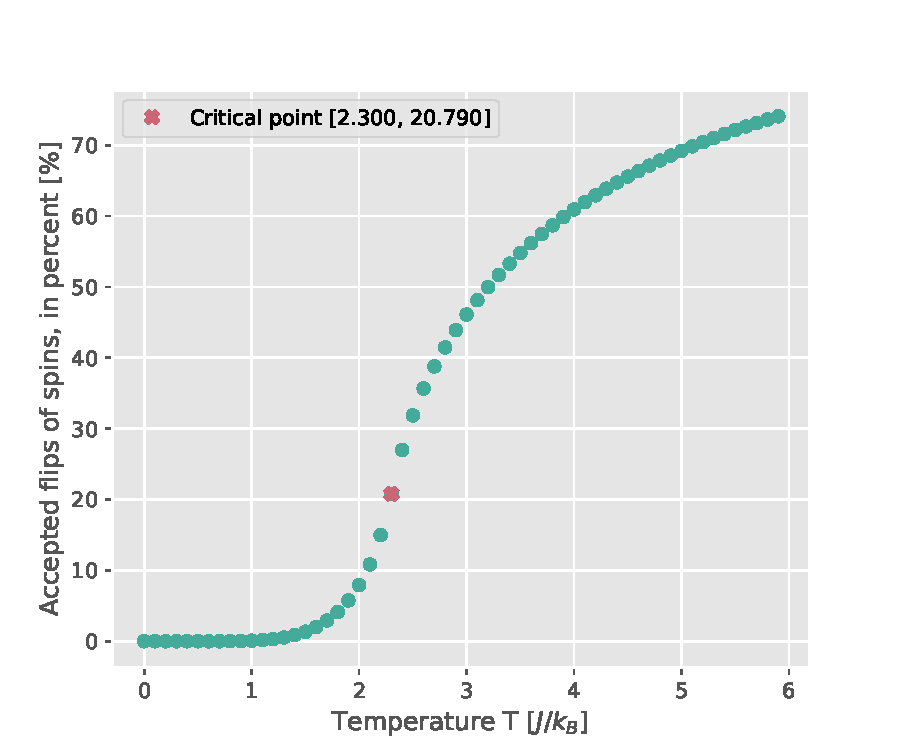
\includegraphics[width = 0.52\textwidth]{figures/20x20acceptflips_t_EXTRAASF.pdf} 
    \caption{Percent of accepted flips (calculated after entire simulation was finished) as a function of temperature for a $20\times 20$ lattice, after $10^6$ Monte Carlo cycles performed by the simulation. Calculated from spins initialized in a random direction. The plot marks the spot where our curve has it's steepest point, [2.300$J/k_B$, 20.790\%].}
    \label{fig:acceptedflips}
\end{figure} 


\begin{figure}[H]
    \centering
    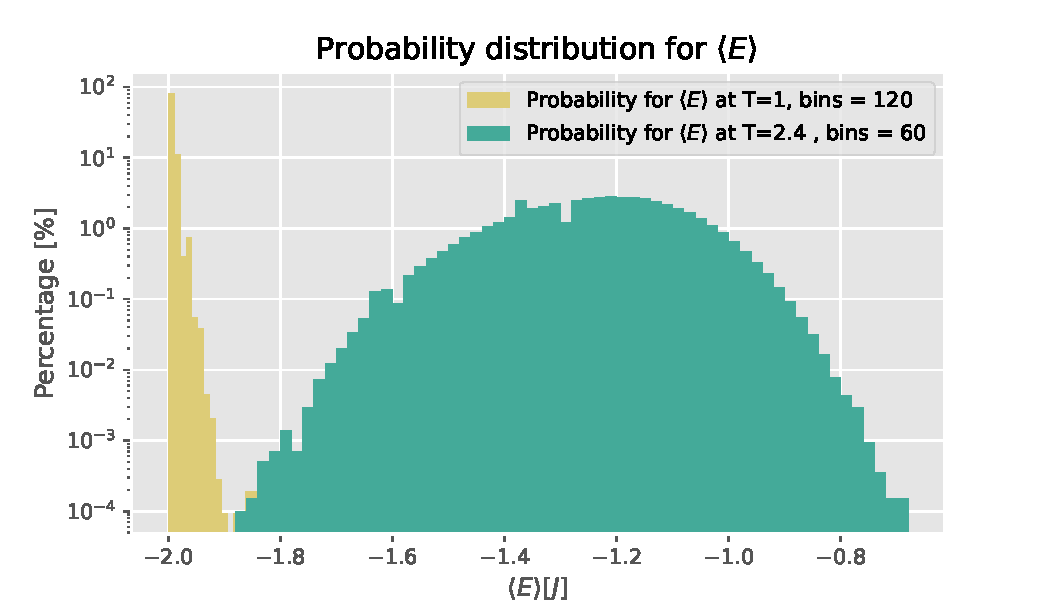
\includegraphics[width = 0.5\textwidth]{figures/20x20prob.pdf} 
    \caption{Probability distribution for $20\times 20$ at $T=1J/k_B$ and $T=2.4J/k_B$, with randomly initiated spins. Count of times each expected energy is obtained/has occurred in our model. Shown as percent, with a logarithmic scaling in the y-axis. Estimated by $10^6$ Monte Carlo cycles.}
    \label{fig:perc}
\end{figure} 
\begin{figure*}
    \centering
    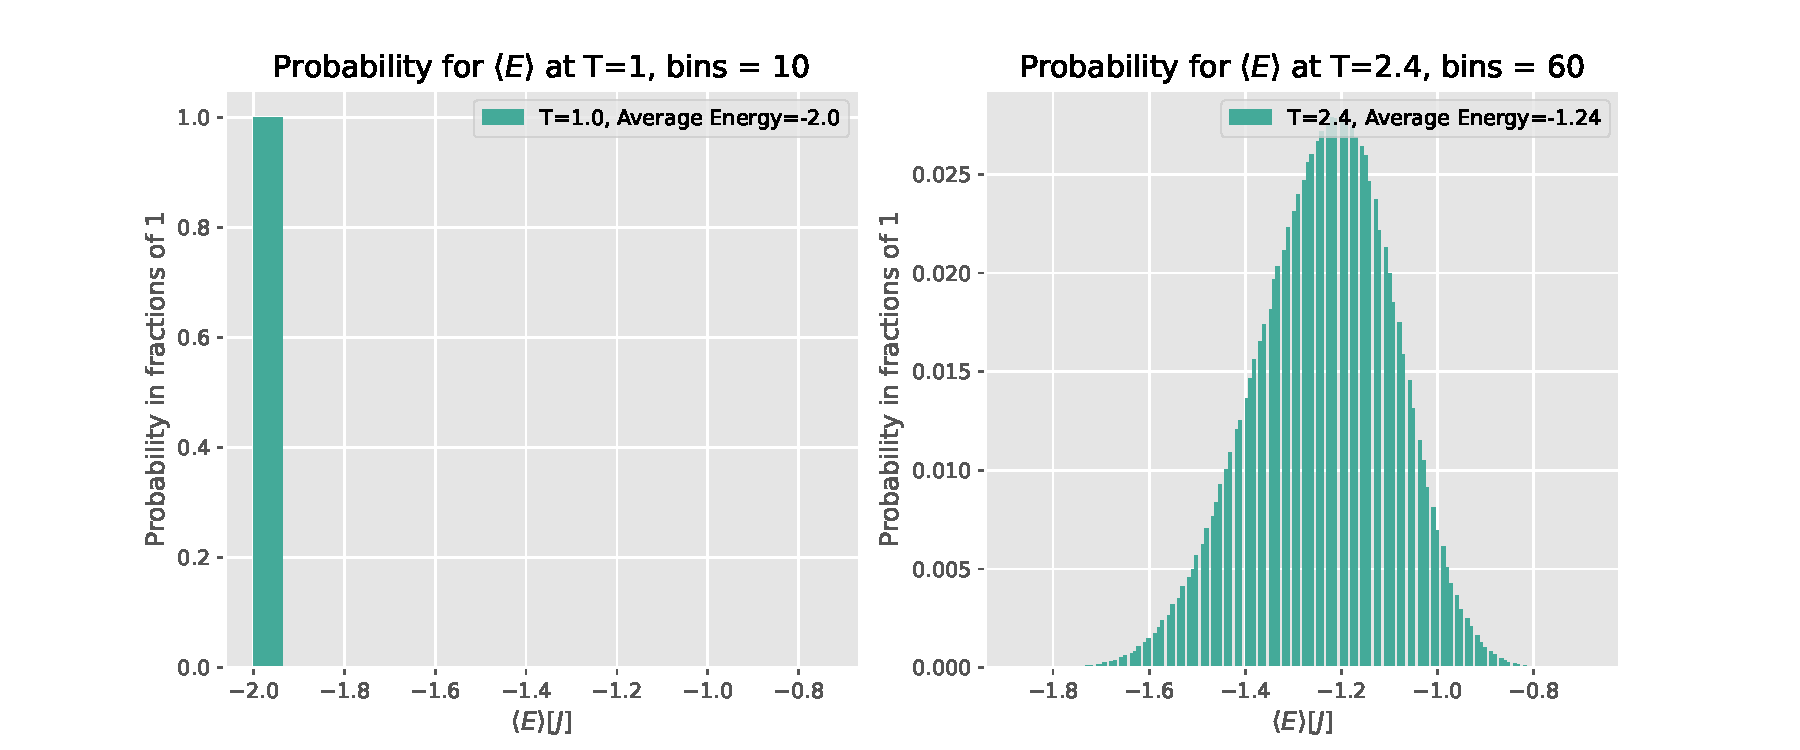
\includegraphics[width = 1\textwidth]{figures/20x20probweighted.pdf} 
    \caption{Probability distribution for $20\times 20$ at $T=1J/k_B$ and $T=2.4J/k_B$, with randomly initiated spins. Count of times each expected energy is obtained/has occurred in our modelled data. Shown as fractions of a whole, 1. Estimated by $10^6$ Monte Carlo cycles.}
    \label{fig:frac}
\end{figure*} 
%Variance in energy for T = 1: 0.02721097750007175
%Standard deviation in energy for T = 1: 0.1649575021030318
%Variance in energy for T = 2.4: 8.161175999999978
%Standard deviation in energy for T = 2.4: 2.856777205173686
\newpage
Figure \ref{fig:frac} can be used to determine the average energy, and correlated variance and standard error for each system. By looking at both figures, one can read an approximate average energy -2.0J for $T=1J/k_B$, and an average energy -1.2J for $T=2.4J/k_B$, and the following values, presented in Table \ref{tab:var}.
\begin{center}
    \begin{table}[H]
    \caption{Variance and standard error for distribution in plots visualized in Figures \ref{fig:frac} and \ref{fig:perc}. Calculated from data obtained when running simulations for $10^6$ Monte Carlo cycles, at temperature $T=1J/k_B$ and $T=2.4J/k_B$, for lattices of size $20\times 20$.}
        \begin{tabular*}{0.5\textwidth}{@{\extracolsep{\fill}}ccc}
        \toprule
        \hline \\
        Temperature T: & Variance: &  Standard deviation in energy: \\
        \midrule
        \hline \\
        \textbf{1$J/k_B$} & 0.0272 &  0.165 \\
        \textbf{2.4$J/k_B$} & 8.161 &  2.857 \\
        \hline
        \bottomrule
        \end{tabular*}\label{tab:var}
    \end{table}
\end{center}


\newpage
\subsection{Varying Sizes of Lattices}
Simulation of behaviour of large lattices is required to study phase transitions for our Ising Model, which is why we perform a parallelization of our code. To show how convenient this usage of parallelized code is, we perform a test modelling behaviour within lattices of varying sizes with $10^5$ MC cycles, with and without usage of parallelized code, and visualize the differences in a Figure \ref{fig:parallel}, as well as in Table \ref{tab:mcctimer}. 

\begin{figure}[H]
    \centering
    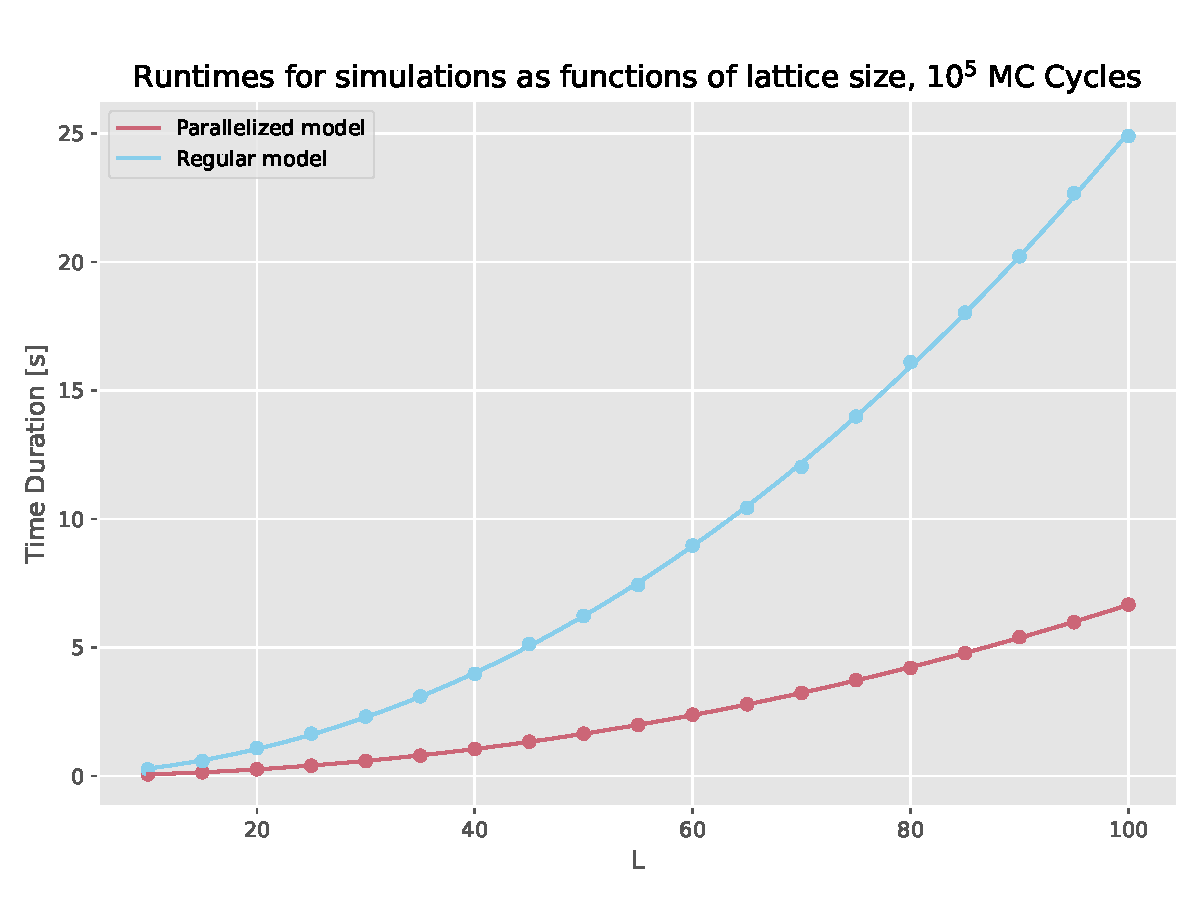
\includegraphics[width = 0.45\textwidth]{figures/duration.pdf} 
    \caption{Comparison of the timing for both the parallelized and non-parallelized code, for $10^5$ amounts of Monte Carlo cycles. The timing is shown as a function of lattice sizes, varying from L=10 to L=100, where a timing test is performed with dL=5. The parallel runs used 4 threads.}
    \label{fig:parallel}
\end{figure} 

\begin{center}
    \begin{table}[H]
    \caption{Performance comparison with $10^5$ Monte Carlo cycles, for parallelized an non-parallelized code. Contains the coordinates of the data points visualized in Figure \ref{fig:parallel}.}
        \begin{tabular*}{0.5\textwidth}{@{\extracolsep{\fill}}ccc}
        \toprule
        \hline \\
        \textbf{L}  & \textbf{Regular [s]} & \textbf{Parallelized [s]} \\
        \midrule
        \hline \\
        10.0 &  0.261 & 0.067 \\
        15.0  & 0.583 & 0.150 \\
        20.0 & 1.089 & 0.263 \\
        25.0 &  1.652 & 0.404 \\
        30.0 & 2.316 & 0.583 \\
        35.0 &  3.103 & 0.797 \\
        40.0 & 3.980 & 1.056 \\
        45.0 &  5.135 & 1.339 \\
        50.0 &  6.235 & 1.648 \\
        55.0 & 7.439 & 1.988 \\
        60.0 &  8.970 & 2.389 \\
        65.0 &  10.437 & 2.792 \\
        70.0 &  12.033 & 3.236 \\
        75.0 &  13.990 & 3.731 \\
        80.0 &  16.104 & 4.209 \\
        85.0 & 18.032 & 4.781 \\
        90.0 & 20.218 & 5.403 \\
        95.0 & 22.673 & 5.984 \\
        100.0 &  24.900 & 6.671 \\
        \hline
        \bottomrule
        \end{tabular*}\label{tab:mcctimer}
    \end{table}
\end{center}
\newpage
\begin{figure*}
    \centering
    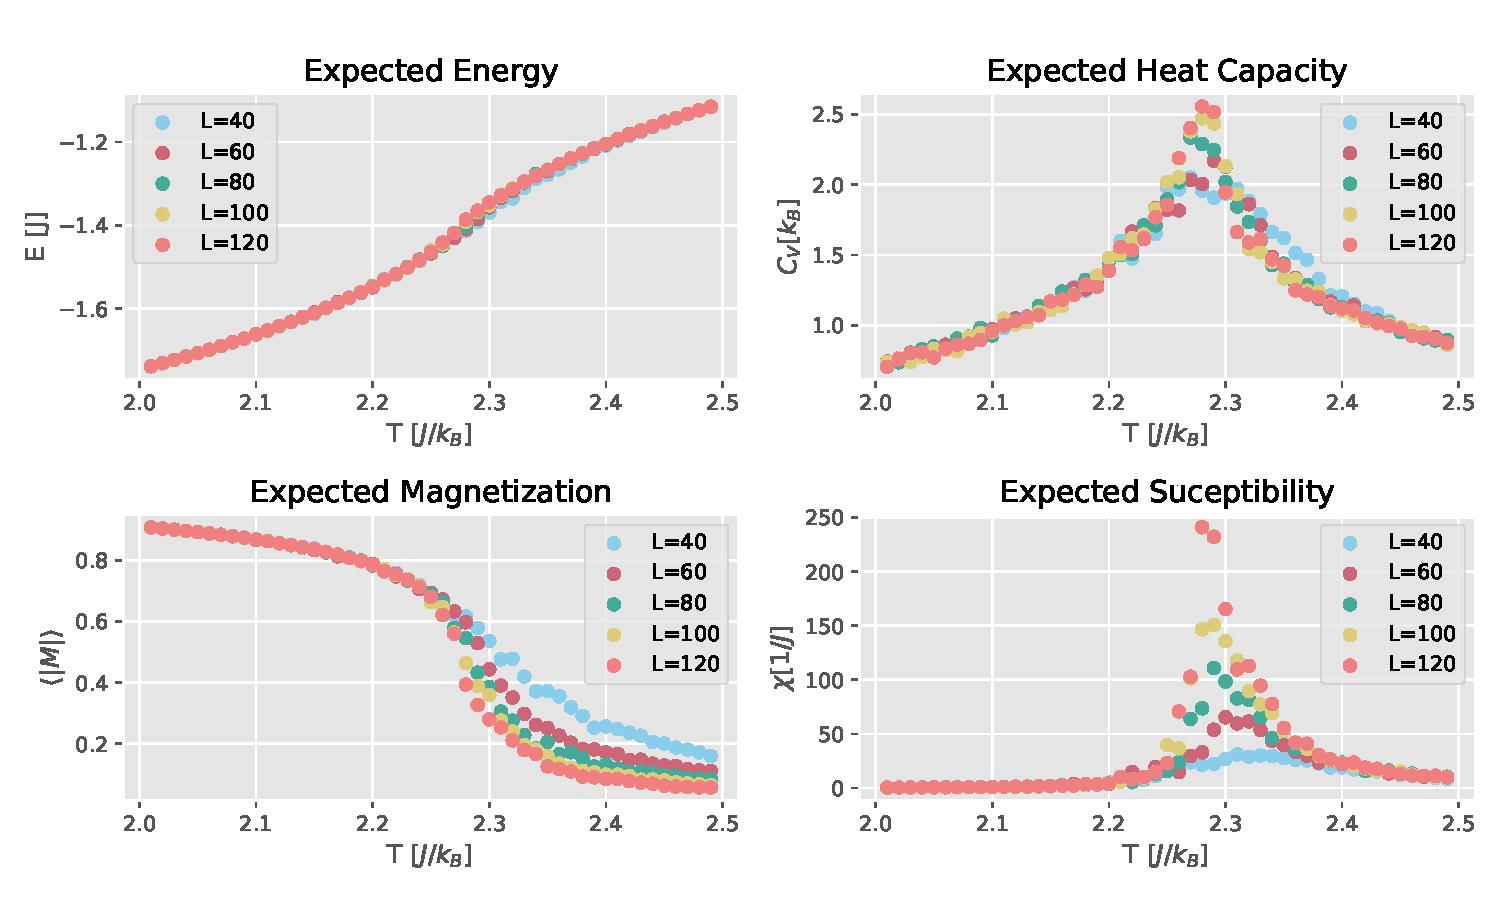
\includegraphics[width = 1\textwidth]{figures/sizevariations.pdf} 
    \caption{Expected energy (top left), absolute magnetization (bottom left), heat capacity $C_V$ (top right) and susceptibility $\chi$ (bottom right) as functions of temperature $T\epsilon [2,2.5]J/k_B$ and dT=0.01$J/k_B$, for lattices of sizes $L\epsilon [40, 60, 80, 100, 120]$. The plots show how the phase transition is dependent on the lattice size. The critical temperature will be where this change is the most drastic, and thereby also where the susceptibility and heat capacity estimations are at a peak. All estimations done by $10^5$ MC cycles.}
    \label{fig:sizevar}
\end{figure*} 
\begin{figure*}
    \centering
    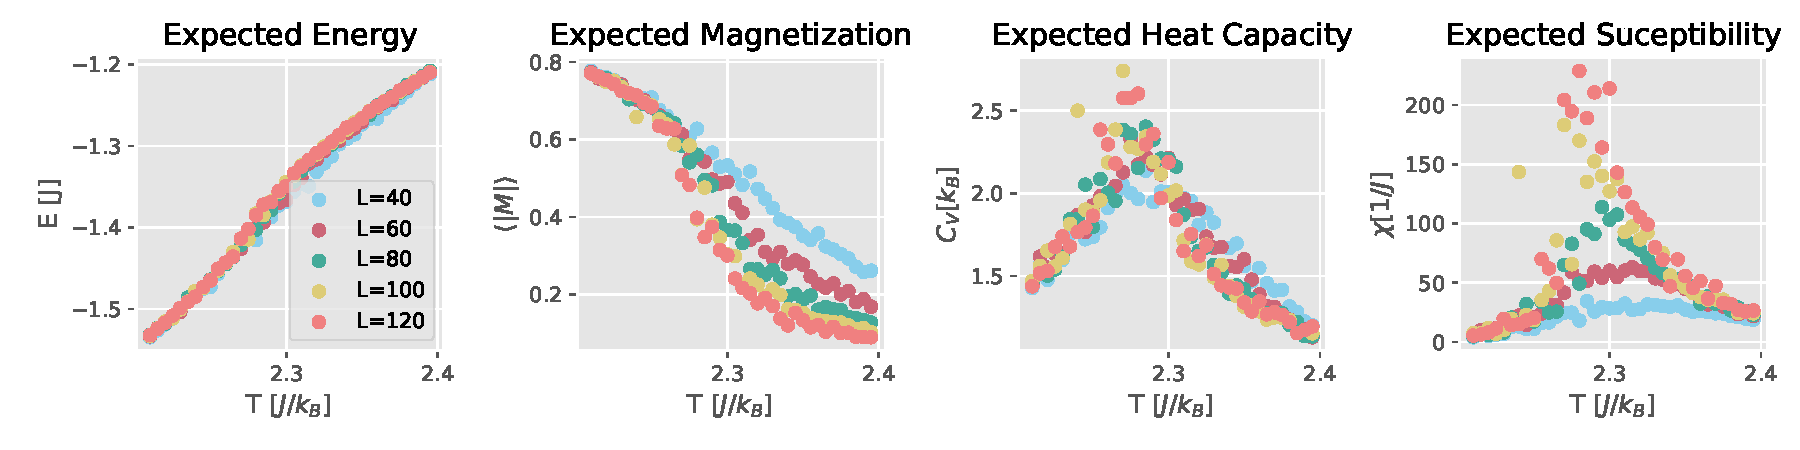
\includegraphics[width = 1\textwidth]{figures/sizevariationszoom.pdf} 
    \caption{Expected energy (far left), absolute magnetization (middle left), heat capacity $C_V$ (middle right) and susceptibility $\chi$ (far right) as functions of temperature $T\epsilon [2.2,2.4]J/k_B$ and dT=0.005$J/k_B$, for lattices of sizes $L\epsilon [40, 60, 80, 100, 120]$. The plots show how the phase transition is dependent on the lattice size. All estimations done by $10^5$ MC cycles, to get more accurate models in a more interesting interval, closer to the critical point. The plots are presented in a (2,2) grid for a closer look, in the Appendix attachment \ref{fig:closerlook}.}
    \label{fig:sizevarzoom}
\end{figure*} 

Furthermore, we study phase transitions by simulating the behaviour of different size lattices at varying temperatures around the critical temperature $T_C$. The sizes of lattices are determined to be $L\epsilon [40, 60, 80, 100, 120]$. For each of these lattice-sizes, the expected values for energy, absolute magnetization, as well as heat capacity and susceptibility is modelled, estimated, and visualized in Figure \ref{fig:sizevar}. By implementing a function that estimates the behaviour of the heat capacity in each instance of lattice-size using the Savitzky-Golay filter like in figure \ref{fig:zoom}, and determining at what temperature this function has its largest value \ref{fig:zoom}, we estimate the critical temperatures $T_C$. These estimations of $T_C$ are compared and merged by linear regression, visualized in Figure \ref{fig:linear}.

\vspace*{2\baselineskip}
\begin{figure}[H]
    \caption{Savitzky-Golay filter applied to the expected heat capacity, in a zoomed in interval - a function estimated to fit the points that were modelled at the different temperatures for the different lattice sizes. All estimations done by $10^5$ MC cycles, by using the data presented in Figure \ref{fig:sizevarzoom}, that is more accurate for the interesting interval. Includes points marking the critical point for each system. The values of these estimated critical temperatures are presented in the Table \ref{tab:tc}.}
    \centering
    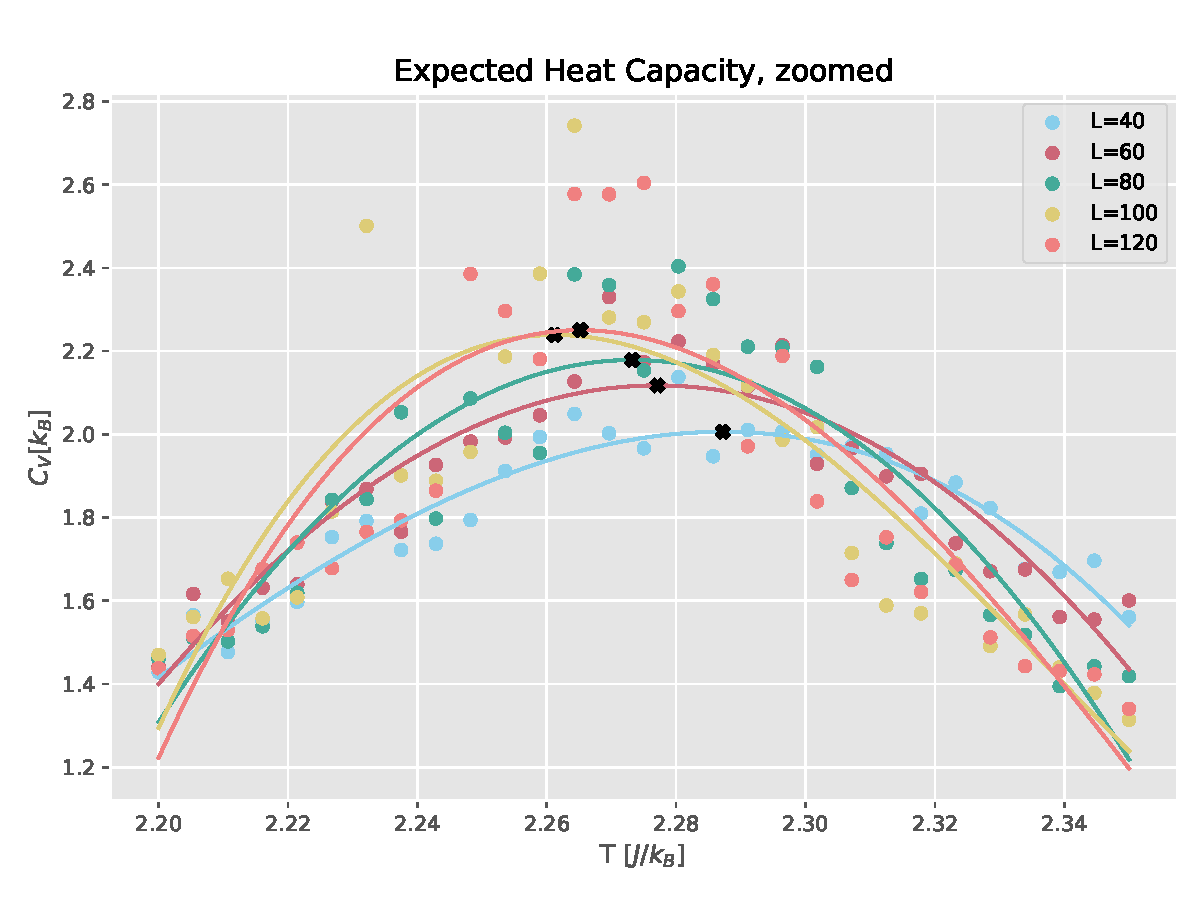
\includegraphics[width = 0.5\textwidth]{figures/heat_capacity_zoom.pdf} 
    \label{fig:zoom}
\end{figure} 

\newpage
\begin{figure}[H]
    \caption{The linear regression implemented to find the best estimation of the critical temperature $T_C$, as well as the data points showing each estimation of the temperature for the lattices of each size. All estimations done by $10^5$ Monte Carlo cycles, and calculated from the data set simulated for the temperature interval $T\epsilon [2.2,2.4]$$J/k_B$ and dT=0.005$J/k_B$. The point where the linear regression intercepts the y-axis is extracted as our best estimation of $T_C$, and the standard error resembles our relative error displayed in the figure.}     
    \centering
    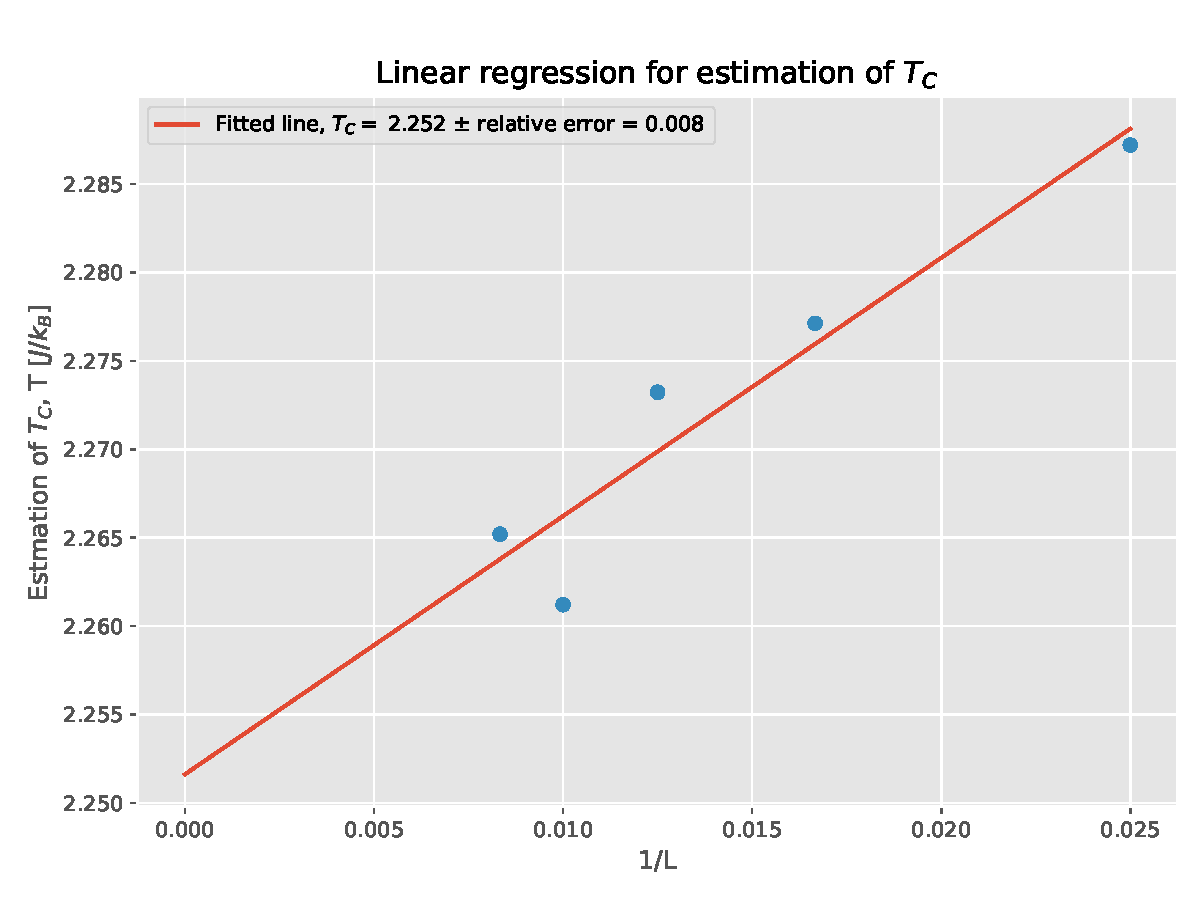
\includegraphics[width = 0.5\textwidth]{figures/linear.pdf} 
    \label{fig:linear}
\end{figure} 
%L:
%[40, 60, 80, 100, 120]
%T_C:
%[2.28720372 2.27712271 2.27322232 2.26120612 2.26519652]
%[ 0.01801872  0.00793771  0.00403732 -0.00797888 -0.00398848]

\begin{center}
    \begin{table}[h]
    \caption{Estimated critical temperature $T_C$ for each lattice-size, visualized in Figure \ref{fig:linear}. Relative error is estimated using the value we know for $T_C=2.269185J/k_B$. Estimated in a temperature interval $T\epsilon [2.2,2.4]$$J/k_B$, with an amount $10^5$ Monte Carlo cycles.}
        \begin{tabular*}{0.5\textwidth}{@{\extracolsep{\fill}}ccc}
        \toprule
        \hline \\
        L: & Estimated $T_C$$[J/k_B]$: &  Relative error: \\
        \midrule
        \hline \\
        40 & 2.28720372 &  0.01801872 \\
        60 & 2.27712271 &   0.00793771\\
        80 & 2.27322232   &  0.00403732 \\
        100 & 2.26120612 &   0.00797888\\
        120 & 2.26519652 &  0.00398848 \\
        \hline
        \bottomrule
        \end{tabular*}\label{tab:tc}
    \end{table}
\end{center}



\cleardoublepage
\section{Discussion}\label{sec:discussion}
\subsection{2x2 Lattice Theory Comparison}
Figure \ref{fig: fig1} shows a comparison between the analytic expectation values for a $2\times 2$ lattice structure (Equations \eqref{eq:anpar} - \eqref{eq:ancritchi2}), and data for the same values collected by our Ising Model calculated by $10^5$ Monte Carlo cycles. Since the lattice is of a very small size, we cannot conclude that the behaviour of the expectation values with change in temperature is applicable for lattices of all sizes, or that it is accurate visualization in the grander scheme. Nevertheless, considering the conformity between the modelled and analytic expectation values, we can conclude that the simulation is working as intended. Figure \ref{fig: fig2} shows us how the accuracy for the data points increase with an increasing amount of performed Monte Carlo cycles, with corresponding values describing the error presented in the table \ref{tab:mcerr}. From the figure and table together, one can see the accuracy increasing a considerable amount with an increasing amount of Monte Carlo cycles performed to estimate the critical point. An amount between $10^4$ and $10^5$ cycles seem from this set of data to be enough to represent the system to an adequate degree of precision. To be sure, though, we need to assess if this is a theory applicable for larger lattices, and more complex systems. \\


\subsection{The 20x20 Lattice}
We used the lattice of size $20\times 20$ to further investigate how many Monte Carlo cycles are needed for the system to reach equilibrium. Figure \ref{fig:cycleamount} shows how both the expected energy and absolute magnetization behaves with an increasing amount of Monte Carlo cycles, from $10-10^6$ for environments where spins are initialized in the same direction, as well as random directions, at temperatures T=1J and T=2.4J. From this Figure, we gather the following: \\

A system at a temperature lower than the critical temperature (low energy) where all spins are in an ordered initial direction, will already be in an equilibrium state. This is due to the energy change when attempting flipping a spin never meeting the requirement of the metropolis algorithm - the spins have only a small chance of actually flipping, due to it's almost nonexistent reason to do so. With the on-average constant energy, comes a constant magnetization, as one can gather from Equation \eqref{eq:mag}. This explains the curve for the system at temperature T=1$J/k_B$ with ordered spins', which is constant at E=-2J and M=1. A low energy system with randomly initiated spins will attempt to obtain the same equilibrium state by flipping spins, until it reaches the same conditions as the system initialized with ordered spins. This is what we see happen for the curves in our plot, for both the magnetization and energy after around $10^4$ Monte Carlo cycles have been conducted. We notice that the curves for the system at random initial spins experiences the largest influx of change right as the simulation starts, and settles as the number of Monte Carlo cycles increases. This is explained by the decreasing probability of flips occurring in our system - as we approach equilibrium, more and more spins become content with their direction of spin. Therefore, the rate of spin-flipping decreases as the simulation runs. \\

The curves for the system at a higher temperature T=2.4$J/k_B$, are more interesting to look at, as it indicates a system of higher disorder. The curves of both the systems of ordered and non-ordered initial spins seem to fluctuate a bit, before stabilizing after about $10^4$ Monte Carlo cycles have been conducted, at energy E=-1.2J and magnetization M=0.45. The fluctuation can be explained by the randomness of our system, increasing the chances for us to flip a spin in both positive and negative energy-change direction. This, we can see in accordance with the Figure \ref{fig:acceptedflips}, which indicates that a significantly larger amounts of flips will occur when the temperature in our system is larger than the critical temperature $T_C\approx 2.27 J/k_B$, than when the system is at a lower temperature. When the system is at a temperature in the interval $T\epsilon [0,1]J/k_B$ with spins initialized in random directions, there seems to be no flips of spins occurring at all. As the temperature increases, the probability of a randomly selected spin flipping also increases. The model has a turning point at T=2.3$J/k_B$ - this is where the shape of our plotted data is the steepest, and thereby also the point where one would expect the most change to happen. This fits well with our theory for the critical temperature, estimated by this figure to be approximately T=2.3$J/k_B$. The inaccuracy in this estimation is more than likely due to the model's inaccuracy in this specific interval $T\epsilon [2,3]J/k_B$. If we created a simulation that approximated the probability of spins to flip in this interval with a greater degree of precision, this point would in theory be closer to the critical temperature $T_C\approx 2.27 J/k_B$.
Ultimately, though, equilibrium is reached at a state where the distribution of flips is 50($\uparrow$)/50($\downarrow$), which is confirmed and emphasised by our probability distribution Figures \ref{fig:perc} and \ref{fig:frac}. \\

These two Figures \ref{fig:perc} and \ref{fig:frac} visualize the probability for a certain system-energy to be measured within the system with randomly initialized spins for both the temperature T=1$J/k_B$ and T=2.4$J/k_B$. The Figure \ref{fig:frac} shows an average energy E=-2J for the system in T=1$J/k_B$, which is in accordance with what we found from the Figure \ref{fig:cycleamount}. For the system with temperature T=2.4$J/k_B$, we find that the most probable state of energy is E=-1.24J, the average energy of expectation energy. This is also the energy our system will possess when it is in a state of equilibrium. From our Table \ref{tab:var}, we can read a substantially larger variance \cite{stats} for a higher temperature, which does mean that the states around the average is more obtainable - it is more likely for a system to exist in any of these energy-states close to the average as the temperature increases. We know this is true, by confirming with our previous finds - for a higher temperature system, the probability of spin flipping is higher, and even as we move closer to equilibrium, the flips keep happening until we eventually reach equilibrium. From this, one can expect a wider distribution function for a system at increasingly higher temperatures. We can also explain this by looking at the Equation \eqref{eq:partitionfunc}; then the temperature T increases, the Boltzmann constant becomes smaller, and the distribution larger. \\ 

We discovered from this experiment, that equilibrium is reached somewhere in the interval $[10^4 , 10^5]$ amounts of Monte Carlo cycles. Subsequently, the rest of the simulations conducted in this report were done for a duration of $10^5$ Monte Carlo cycles, to make sure equilibrium was reached. This state being reached is of great importance, as we want to obtain the most reliable estimations of expectation values as possible, as close to the critical point as possible.


\subsection{Parallelization}
We perform a test showing how much more efficient a use of parallelized code is, and present the results in Figure \ref{fig:parallel}. From this plot we can read a clear advantage in making use of the method when dealing with larger size lattices, from the run-time difference of about $\frac{24.9}{6.671}=3.73\approx 4$, by values presented for lattice of size L=100 in the Table \ref{tab:mcctimer}, which is expected as we used 4 threads for our parallelized simulation. This is a tremendous advantage, that we did make use of when running the following simulations for the varying size lattices. 


\subsection{Varying Sizes of Lattices}
Figure \ref{fig:sizevar} visualizes how estimated expectation values changes as functions of both temperature T in the interval $T\epsilon [2.0,2.5]J/k_B$, and the size of the lattice L. The Figure \ref{fig:sizevarzoom} gives us a closer look at the more interesting interval, $T\epsilon [2.2,2.4]J/k_B$, where we can see a clear maximum value for both the heat capacity and magnetic susceptibility around the critical temperature, for all the sizes of lattices we created models for $L=[40,60,80,100,120]$. This is expected for the heat capacity, and we take advantage of this to estimate the accuracy of our model. Figure \ref{fig:linear} and table \ref{tab:tc} shows how the critical temperatures calculated from our the modelled heat capacities for the different size lattices increases in accuracy, as the modelled lattice increases in size, by taking advantage of the correlation between lattice-size and critical temperature expressed by the Equation \eqref{eq:corr}, and perform a linear regression. On average, the modelled value for critical temperature turns out to be $2.252 \pm 0.008 J/k_B$, which is very accurate, and thereby we can conclude that this theory for phase transitions does describe the behaviour observed for our model near the critical temperature. Uncertainties in this instance would be a result of the method we used to model a function best fitted to our heat capacity data. This uncertainty was attempted to keep as negligible as possible, by running simulations for smaller temperature steps in the immediate temperature interval around the critical temperature.\\
One would expect an immediate diverging behaviour for the magnetic susceptibility around the critical point for an infinitely large lattice, but since we're dealing with lattices of finite sizes, we do not observe this behaviour in our plot. Nevertheless, one can clearly see that there is a difference in the speeds in which the magnetic susceptibility approaches the state of M=0 for temperatures $T>T_C$; the larger the lattice is, the faster it does approach M=0. This is in agreement with our theory for the behaviour during phase transitions, and as expected. Moreover, the plot visualizing energy development as a function of temperature in Figure \ref{fig:sizevarzoom}, does not display any large differences in behaviour dependent on the size of our lattice. There seems to be a small difference in behaviour in a small interval at and after the critical temperature, which quickly aligns again after. The magnetization and magnetic susceptibility both have an obvious lattice size-dependence, which is in line with the relations described by the Equations \eqref{eq:relations}. The data modelling the expected magnetisation seem to be steeper for a larger lattice, which is also consistent with this relation; a larger value L lattice size will result in a larger denominator in our fraction describing the relations. The expected magnetization is also dependent on temperature; an increase in temperature within our system also contributes to the decrease in the expectation value, which is behaviour we see occurring in our model.
These relations also explain the relation heat capacity has to the lattice size around the critical point. When seeing the behaviour of the energy as functions of temperature and lattice size in the light of this relation for heat capacity, as well as the energy-dependent expression for heat capacity Equation \eqref{eq:heat}, this could explain the behaviour of the energy we observe in our plots.

\cleardoublepage
\section{Conclusion}\label{sec:conclusion}
The 2D Ising model was implemented by making use of the Monte Carlo based Metropolis algorithm, by developing a c++ script. The model, describing an $L\times L$ lattice structure with boundary conditions containing N spins $s_i$, was used to study phase transitions. To make sure our model was implemented correctly and producing results with an appropriate degree of precision, we compared data accumulated when simulating the behaviour of a $2\times 2$ lattice with analytically derived expressions, and found an excellent conformity. We ran tests examining to what extent the Metropolis algorithm would have to be used for the system to reach equilibrium, by both simulating the $2\times 2$ with varying amounts of Monte Carlo cycles performed, and looking at the behaviour of expectation values for different $20\times 20$ lattices as functions of Monte Carlo cycles. We saw that for ordered states at temperatures lower than the critical temperature, equilibrium was reached almost instantaneously. For other systems on the other hand, with temperatures higher than the critical temperature and both with randomized and ordered initial states of spins, we found a development of expected energy and magnetization that described a system with higher probabilities for spin-flips occurring. This resulted in a fluctuating curve, that eventually stabilized at the state of 50($\uparrow$)/50($\downarrow$) after about $10^4-10^5$ Monte Carlo cycles. We noticed that this was applicable to systems at lower temperatures as well. For the following simulations, we made use of $10^5$ cycles to be absolutely certain the state of equilibrium was achieved for our systems.

We ran simulations investigating the behaviour of systems of different size lattices by making use of parallelized code, and found a good agreement when comparing these results to phase transition theory and temperature-lattice size relations. This data was used to estimate the critical temperature, in which we got $T_{C(estimated)} =2.252 \pm 0.008 J/k_B$, that we see when compared to the critical temperature $T_C=2.269185J/k_B$, has a high degree of accuracy. 

We can conclude that our model will produce simulations with a high reliability and accuracy, as long as it is ran for an adequate amount of Monte Carlo cycles, $10^5$. 


\bibliographystyle{plain}
\bibliography{references4}


\cleardoublepage
\section{Appendix}\label{sec:appendix}
\subsection{Ising model of a $2\times 2$ lattice structure}\label{sec:isingmodel}
A lattice structure with shape $2\times 2$ will contain 4 different spins, that all can exist in only two conditions, $\uparrow$ or $\downarrow$ . We can visualize these structures for a few states: \\
\begin{center} ------------------------------------------------------------ \end{center}
\[\begin{array}{c}
\text{4 spins $+1$} \\
\begin{bmatrix}
\uparrow & \uparrow \\
\uparrow & \uparrow
\end{bmatrix}
\end{array}
\quad
\begin{array}{c}
\text{3 spins $+1$} \\
\begin{bmatrix}
\uparrow & \uparrow \\
\uparrow & \downarrow
\end{bmatrix}
\end{array}\]
\[\begin{array}{c}
\text{2 spins $+1$} \\
\begin{bmatrix}
\uparrow & \uparrow \\
\downarrow & \downarrow
\end{bmatrix}
\end{array}
\quad
\begin{array}{c}
\text{1 spin $+1$} \\
\begin{bmatrix}
\uparrow & \downarrow \\
\downarrow & \downarrow
\end{bmatrix}
\end{array}
\quad
\begin{array}{c}
\text{0 spins $+1$} \\
\begin{bmatrix}
\downarrow & \downarrow \\
\downarrow & \downarrow
\end{bmatrix}
\end{array}\]
\begin{center} ------------------------------------------------------------ \end{center}
The system will have $4^2$ states of existence. We describe each unique state in the following Table \ref{tab:states}:
\begin{center}
\begin{table}[h!]

\caption{Calculations of energies, magnetization and degeneracy of the unique states for a $2\times 2$ lattice.}
\begin{tabular*}{0.5\textwidth}{@{\extracolsep{\fill}}cccc}
\toprule
\hline \\
Spins in State +1 & $E_{\text{tot}}$ & $M_{\text{tot}}$ & Degeneracy \\
\midrule
4 & -8J & 4 & 1 \\
3 & 0 & 2 & 4 \\
2 & 0 & 0 & 4 \\
2 & 8J & 0 & 2 \\
1 & 0 & -2 & 4 \\
0 & -8J & -4 & 1 \\ \\
\hline
\bottomrule
\end{tabular*}\label{tab:states}
\end{table}
\end{center}

\subsection{Deductions of analytical values for a $2\times 2$ lattice structure}
Following are the deduction of our expressions, \eqref{eq:anpar}, \eqref{eq:anene},\eqref{eq:anene2},\eqref{eq:anmag},\eqref{eq:anmag2},\eqref{eq:ancritchi},\eqref{eq:ancritchi2}, regarding the special case of a 2x2 lattice size: \\
To express \(Z\), Eunction \eqref{eq:partitionfunc},  we call the Equation \eqref{eq:partitionfunc}, rewrite, and find 
\[Z = \sum_{i}^{16}e^{-E_i/k_BT} = \sum_{i}^{16}e^{-E_i\beta}\]
\[=e^{-8J\beta} + e^{-8J\beta} + e^{0} + e^{0} = 4e^{-8J\beta} + 12\]
which is an expression that can be rewritten 
\[Z=4cosh(8J\beta)+12\]
We call the Equation \eqref{eq:ene}, and find the expression for \(\langle E \rangle\), Equation \eqref{eq:anene}, our specific case
\[\langle E \rangle = \frac{1}{Z}\left(8J \cdot e^{-8J\beta} + 8J \cdot e^{-8J\beta} + 0 \cdot e^{0} + 0 \cdot e^{0}\right)\]
\[\langle E \rangle = \frac{16J e^{-8J\beta}}{Z} = \frac{-32J\sinh{\left(8J\beta\right)}}{Z}\]
The same procedure is followed for the case of \(\langle E^2 \rangle\), Equation \eqref{eq:anene2}:\\
\[\langle E^2 \rangle = \frac{1}{Z}\left((8J)^2 \cdot e^{-8J\beta} + (8J)^2 \cdot e^{-8J\beta} + 0^2 \cdot e^{0} + 0^2 \cdot e^{0}\right)\]
\[\langle E^2 \rangle = \frac{256J^2\cosh{\left(8J\beta\right)}}{Z}\]
We express \(\langle \abs{M} \rangle\), Equation \eqref{eq:anmag}, by making use of the Equation \eqref{eq:mag}, and find for our \(2\times 2\) lattice 
\[\langle \abs{M} \rangle = \frac{1}{Z}\left(4 \cdot 4 \cdot e^{-8J\beta} + 4 \cdot 4 \cdot e^{-8J\beta} + 4 \cdot 8 \cdot e^{0} + 4 \cdot 8 \cdot e^{0}\right)\]
\[\langle \abs{M} \rangle = \frac{64 + 64e^{8J\beta}}{Z} = 8\frac{2 + e^{8J\beta}}{Z}\]
The same procedure is followed for the case of \(\langle M^2 \rangle\), Equation \eqref{eq:anmag2}:\\
\[\langle M^2 \rangle = \frac{1}{Z}\left(4^2 \cdot 4 \cdot e^{-8J\beta} + 4^2 \cdot 4 \cdot e^{-8J\beta} + 8^2 \cdot e^{0} + 8^2 \cdot e^{0}\right)\]
\[\langle M^2 \rangle = \frac{256 + 256e^{8J\beta}}{Z} = 32\frac{1 + e^{8J\beta}}{Z}\] \\
Subsequently, these analytical expressions can be used to express heat capacity and magnetic susceptibility: 
The heat capacity \(C_V\), Equation \eqref{eq:heat}:
\[C_V = \frac{1}{k_B T^2}\left(\frac{256J^2\cosh{\left( 8J\beta \right)}}{Z} - \left(\frac{-32J\sinh{\left( 8J\beta \right)}}{Z}\right)^2\right)\]
The magnetic susceptibility \(\chi\), Equation \eqref{eq:sus}:
\[\chi = \frac{1}{k_B T}\left(32\frac{1+e^{8J\beta}}{Z} - \left(8\frac{2+e^{8J\beta}}{Z}\right)^2\right)\]

\clearpage
\subsection{Additional plots}\label{sec:plots}
\begin{figure}[H]
    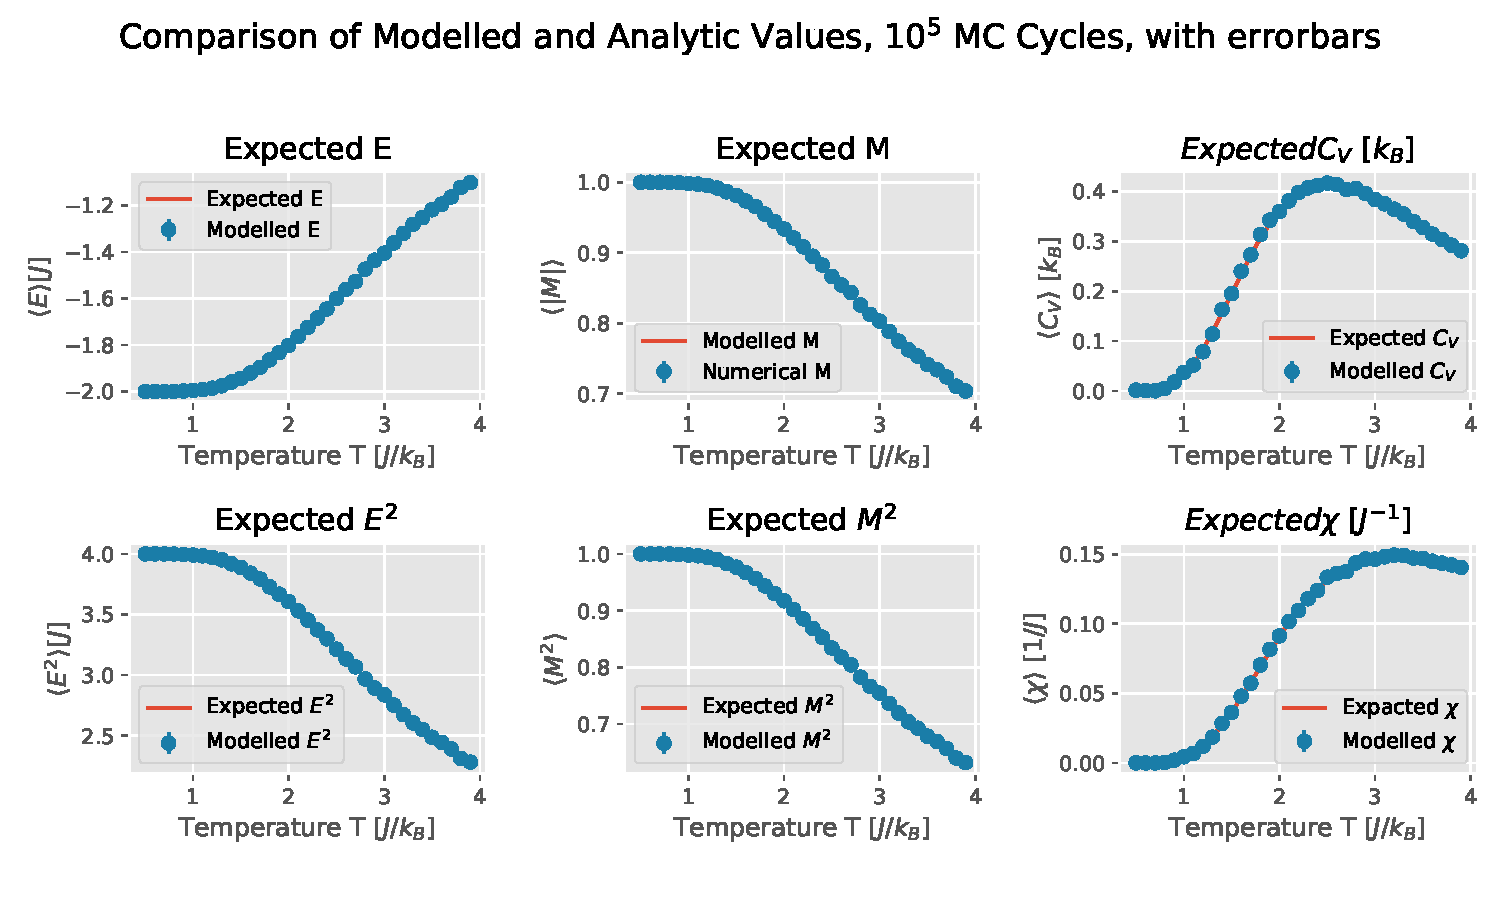
\includegraphics[width = 1\textwidth]{figures/expected_values_errors.pdf} 
    \caption{Shows the estimated expectation values for the 2x2 lattice, compared to our analytic expressions. Visualizing and comparing the numeric and analytic estimation for the expectation values in the special case of a $2\times 2$  lattice, for an amount $10^5$ of Monte Carlo cycles, over an interval of temperature $T\epsilon [0.5,4]J/k_B$ with temperature steps dT=0.1$J/k_B$. Analytic expressions presented by Equations \ref{eq:anpar} - \ref{eq:ancritchi2} in section \ref{sec:analytical}. Including error-bars.}
    \label{fig: fig1errors}
\end{figure} 

\begin{figure*}
    \centering
    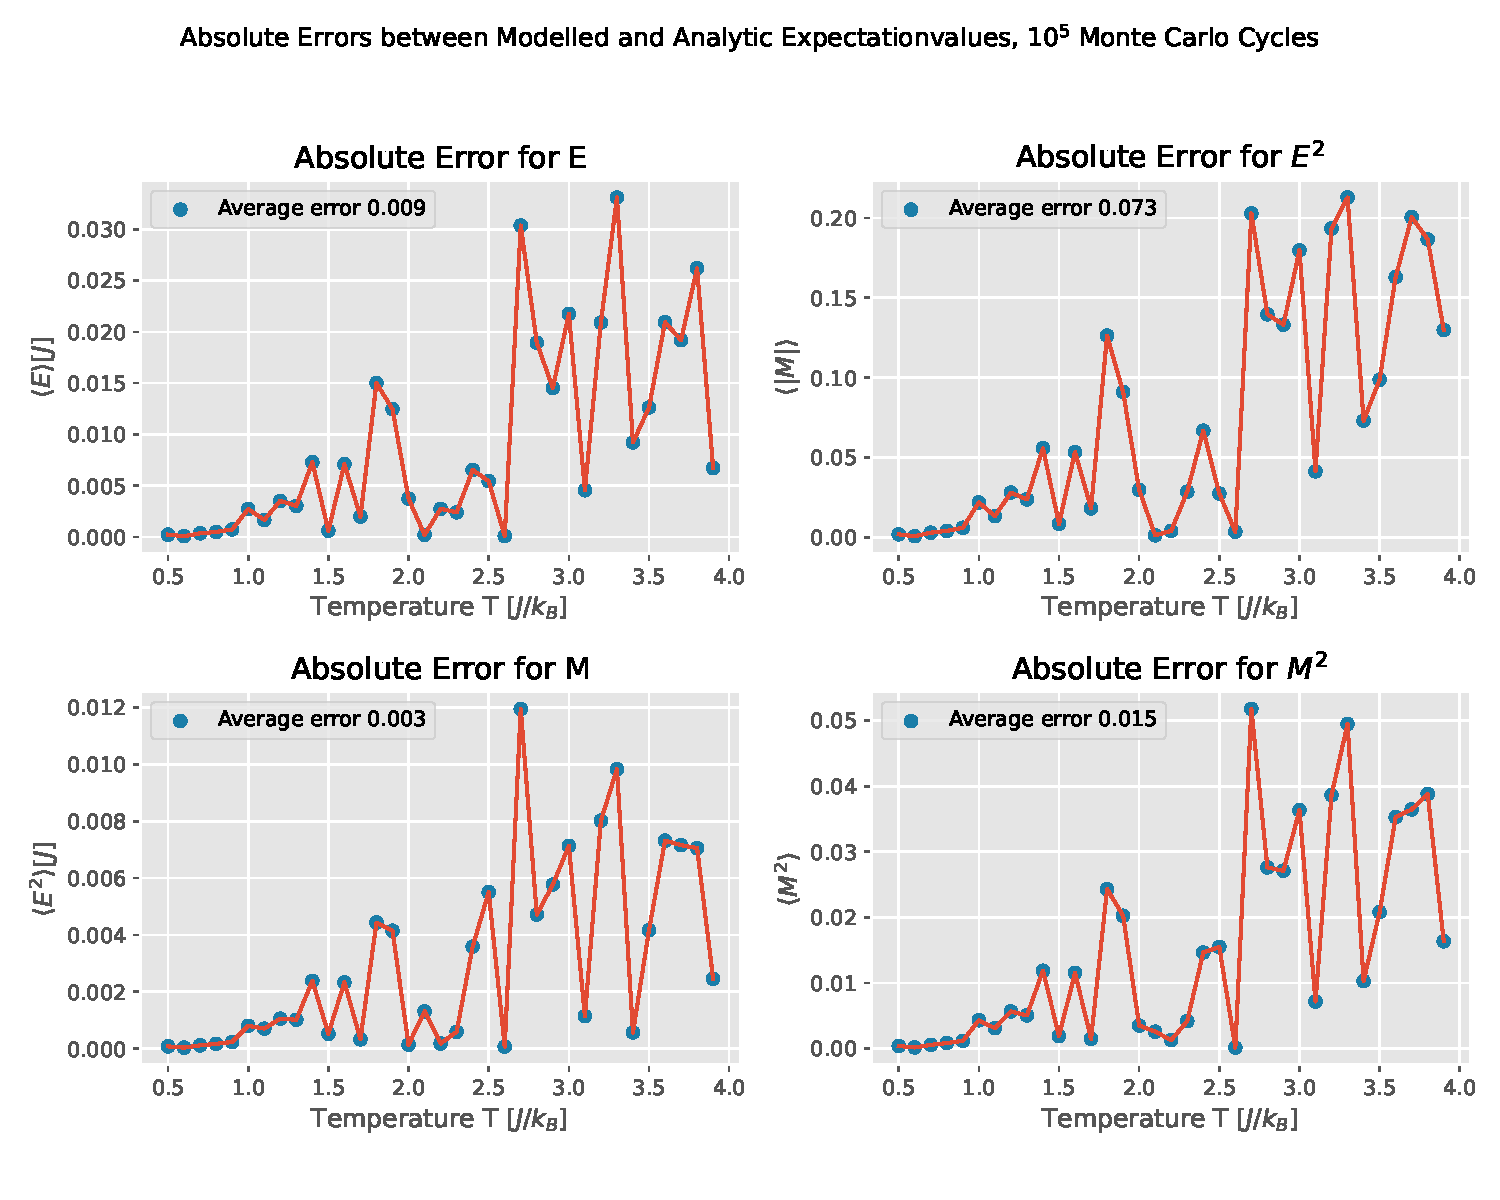
\includegraphics[width = 1\textwidth]{figures/only_errors.pdf} 
    \caption{Showing only the errors in Figure \ref{fig: fig1} and Figure \ref{fig: fig1errors}. The errors show a spike around the critical temperature, which is accurate considering this is where the most abrupt changes in behaviour take place.}
    \label{fig: fig1onlyerrors}
\end{figure*} 

\begin{figure*}\label{fig:all}
    \centering
    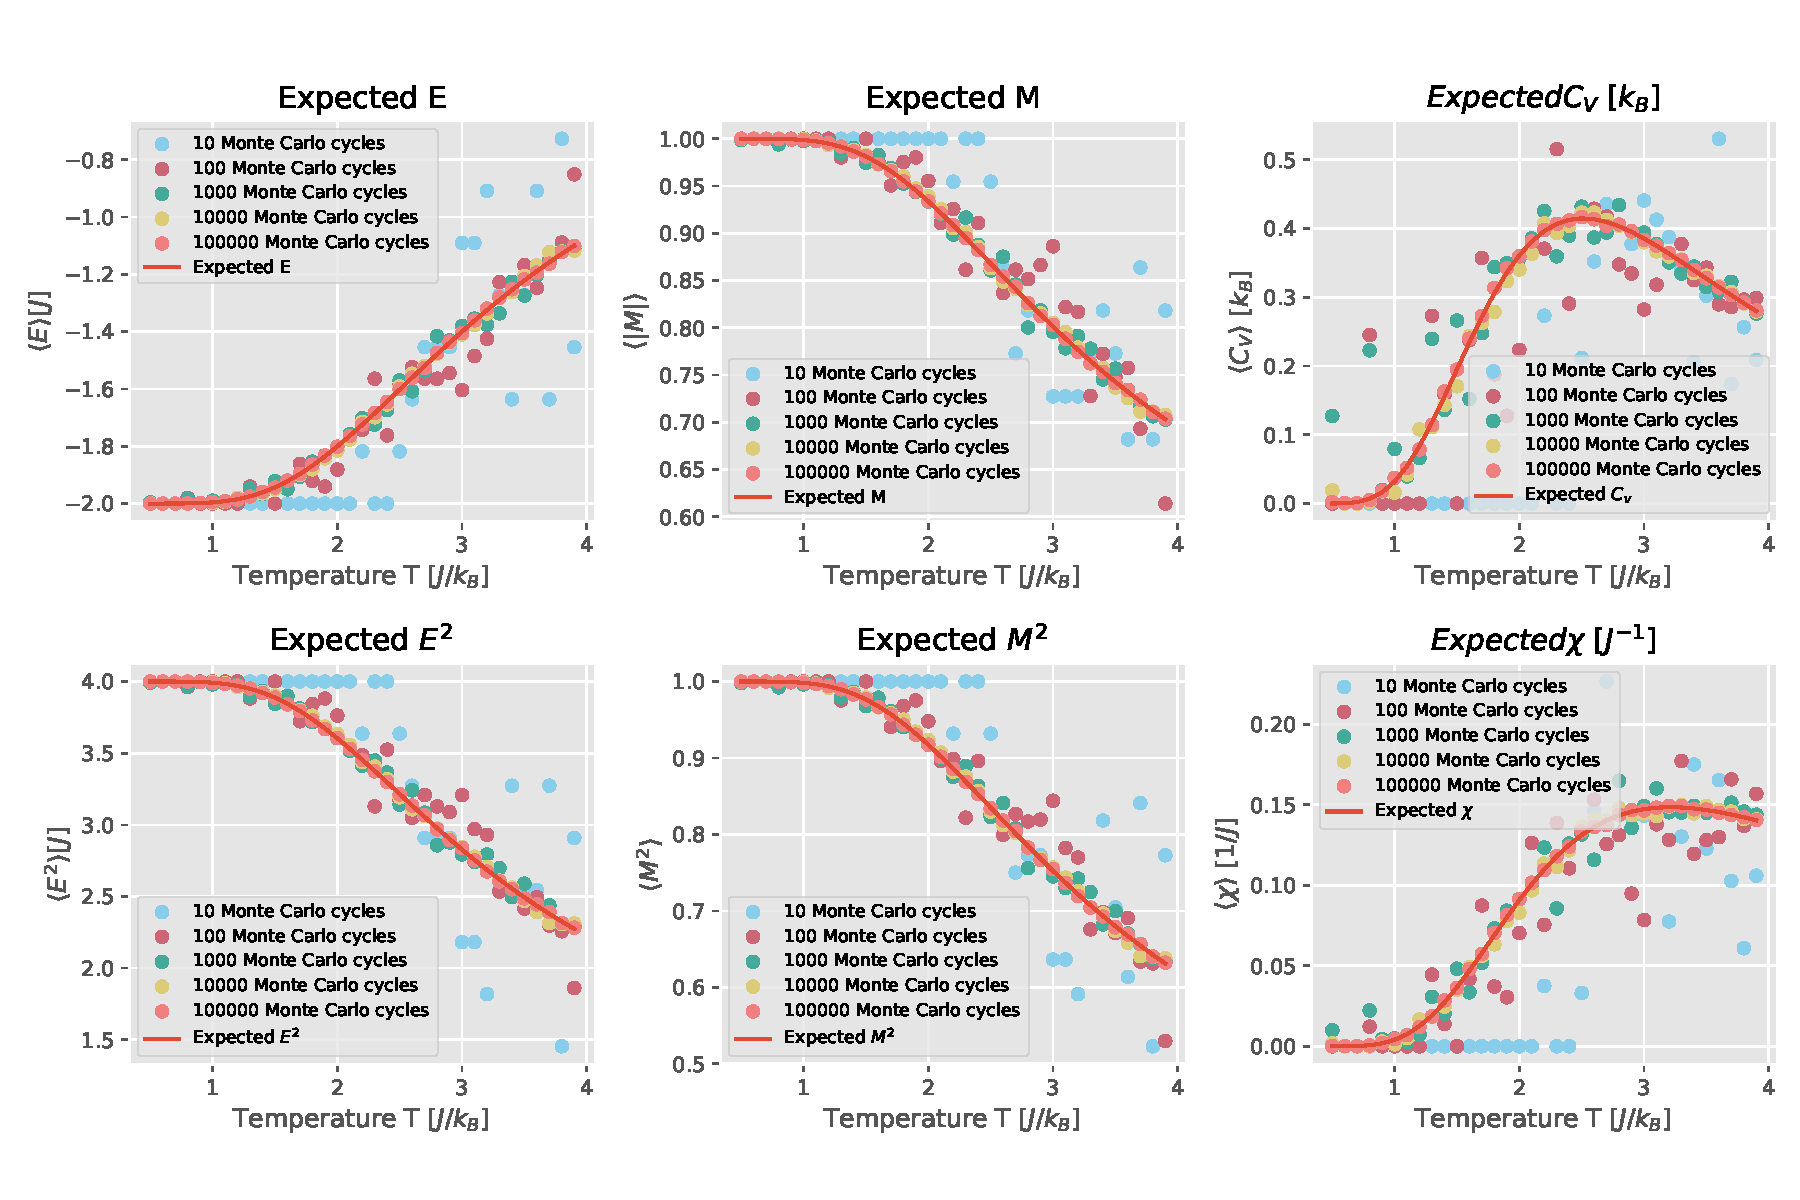
\includegraphics[width = 1\textwidth]{figures/mcc_comp_all.pdf} 
    \caption{Degree of precision for the expectation values of energy ( top left), absolute magnetization (top middle), heat capacity (top right), $E^2$ (bottom left), $M^2$ (bottom middle) and the susceptibility (bottom right) for varying amounts of Monte Carlo Cycles used for estimations. The expectation values are estimated over an interval of temperature $T\epsilon [0.5,4]J/k_B$ with temperature steps dT=0.1$J/k_B$.}
    \label{fig:all}
\end{figure*} 

\begin{figure*}
    \centering
    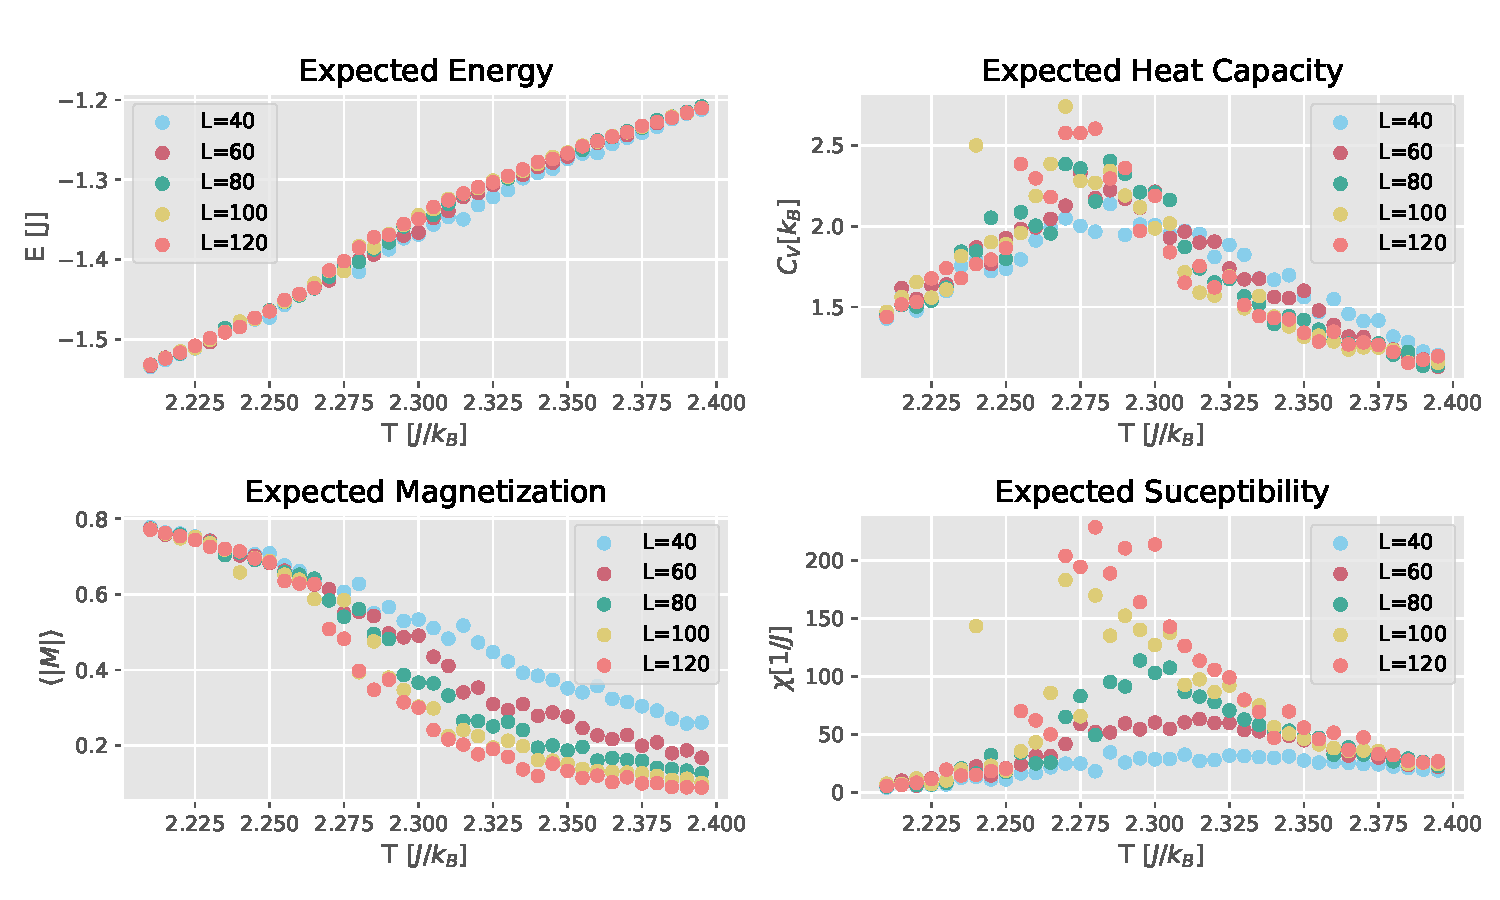
\includegraphics[width = 1\textwidth]{figures/sizevariationszoom4.pdf} 
    \caption{Visualizing expected energy (top left), absolute magnetization (top right), heat capacity (bottom left) and susceptibility (bottom right) as functions of temperature $T\epsilon [2.2,2.4]J/k_B$ and dT=0.005$J/k_B$, for lattices of sizes $L\epsilon [40, 60, 80, 100, 120]$. The plots show how the phase transition is dependent on the lattice size. All estimations done by $10^5$ MC cycles, to get more accurate models in a more interesting interval, closer to the critical point. A closer look at each of the plots in Figure \ref{fig:sizevarzoom}.}
    \label{fig:closerlook}
\end{figure*} 

\end{document}